\documentclass{ctuthesis}
\usepackage{mathtools}
\usepackage{subfig}
\usepackage{xcolor}
\usepackage{listings}
\usepackage{xparse}
\usepackage{siunitx}
\usepackage{psvectorian}
\usepackage{algpseudocode}
\usepackage{verbatim}


\lstset{language=C,keywordstyle={\bfseries \color{blue}}}


\ctusetup{
	xdoctype = B,
	xfaculty = F3,
	mainlanguage = english,
	secondlanguage = czech,
	title-english = {Planning routes for recreational cycling},
	title-czech = {Plánování tras pro rekreační cyklistiku},
	department-english = {Department of Computer Science},
	author = {Miroslav Matocha},
	supervisor = {doc. Ing. Michal Jakob, Ph.D.},
	supervisor-address = {Fakulta elektrotechnická, Resslova 307/9, Praha},
	month = 5,
	year = 2019,
	day = 24,
	keywords-english = {route planning, cycles, cycling, graph search},
	keywords-czech = {plánování cest, cykly, cyklistika, prohledávání grafu}
}

\ctuprocess
\begin{abstract-english}
Using bicycle rides as a leisure activity is very widespread these days. Most of the cycling-focused applications offer planning methods that are great to use when traveling from place to place but are not useful when planning routes suitable for recreational cycling. That's why I decided to propose and implement a solution that would offer planning of such tours. I did a thorough research of papers with a similar scope. Then I chose one of them, which was focused on planning closed routes, and I implemented and modified it for my problem. To achieve this, I defined the problem of planning recreational tours formally. Then I described components necessary for its solution, for example, tour pleasantness and roundness. Next, I covered the solution itself, drawn from the mentioned paper, but extended to plan point-to-point recreational routes as well as closed ones. I identified weak points of the solution and created a modified version where they were targeted. Moreover, I implemented both solutions in Java and created a web service on top of them. The web service comes together with a client which can demonstrate capabilities of these algorithms to the user. The last section is dedicated to experiments that are comparing the solutions of the original application with the modified one and identifying their differences. These experiments have shown that there is not any significant difference in the quality of results from the modified version of the algorithm. However, there is a significant improvement in the overall running time.
\end{abstract-english}
\begin{abstract-czech}
Rekreační jízda na kole se v poslední době stává čím dál více rozšířenou kratochvílí. Většina cykloaplikací nabízí plánování, které funguje skvěle pro nejkratší cestu z bodu do bodu, ale pro plánování rekreačních tras se moc nehodí. Proto jsem se rozhodl vytvořit řešení, které by tyto trasy nabízelo. Udělal jsem důkladný průzkum prací s podobnou tématikou. A poté jsem z nich jednu, která se zabývá plánováním okružních výletů, vybral, abych ji implementoval a modifikoval pro svůj problém. Musel jsem kvůli tomu tento problém formálně definovat. Poté jsem popsal komponenty potřebné k jeho řešení, jako je příjemnost a kulatost těchto tras. Dále jsem rozebral samotné řešení, které se inspirovalo zmíněnou prací a rozšířil ho kromě okruhů i na rekreační trasy z bodu do bodu. Později jsem identifikoval jeho slabiny a vytvořil upravenou verzi řešení, kde se na ně zaměřuji.  Navíc jsem implementoval obě řešení v Javě a vytvořil nad nimi webovou službu, společně s klientem, který může jejich možnosti demonstrovat uživateli. Poslední část je věnovaná experimentům, které mají za úkol porovnat obě řešení a pojmenovat jejich rozdíly. Tyto experimenty ukázaly, že výsledky modifikovaného algoritmu nejsou výrazně odlišné od původní verze. Nicméně, algoritmus zaznamenal výrazné zlepšení v oblasti časové náročnosti.
\end{abstract-czech}


% Acknowledgements / Podekovani
\begin{thanks}

\begin{equation}
\frac {l(\rho_{s \rightarrow t})} {d_{real}(g, t)} \in I
\end{equation}


	At first I have to thank my supervisors Michal Jakob and especially Pavol Žilecký for their patience and for bearing with me throughout this whole process. A big thanks goes also to all of the Umotional company.\par
	I also greatly appreciate the help of Pieter Stroobant. He has gladly answered my questions about his paper and its implementations, which I am very grateful for.\par
	Martin Dolsky and Jan Kalina also deserve an acknwoledgement for proofreading, feedback and very helpful insights.\par
	My last thanks goes, of course, to my family, partner and CTU, for preparing me for and supporting me on this path.
\end{thanks}

% Declaration / Prohlaseni
\begin{declaration}
	I declare that I wrote this paper by myself and that I mentioned all used literature in bibliography section.
	
	In Prague, \ctufield{day}.~\monthinlanguage{title}~\ctufield{year}
\end{declaration}

\NewDocumentCommand{\codeword}{v}{
\texttt{\textcolor{blue}{#1}}
}




\begin{document}
\maketitle
\chapter{Introduction}
\section{Motivation}
Cycling is a way of transport which has been here for almost exactly 200 years\cite{history} now, and in the last years, it experienced very rapid growth because of numerous factors. \par It is a convenient, cheap and most of all environment-friendly way to get yourself around on a shorter distance. These are also the reasons why governments and municipalities support this movement.\cite{uk}\cite{eu} And that is a significant boost to it. We can see the road network improving rapidly by the construction of more and more roads with a dedicated lane for cyclers or even standalone cycleways. This improves the comfort of cycling and attainability of various areas. Lastly, we can also witness a major technical boom in this sector, which reflects itself in various bicycle related applications as well as in the improvements of the vehicle itself. \par
These circumstances that are listed above also contribute to the expansion of recreational cycling among people. By recreational cycling, in this context, we mean riding a bike not to get only from point A to B by the shortest path possible but for the pleasure from the riding itself or to get your daily dose of physical activity. There are numerous ways to use the bike in this manner, ranging from a healthy workout routine up to the exploration of the landscape by wandering through the country on your bike. \par
A large portion of the people is nowadays used to use GPS based navigation as a part of their daily routine in almost every aspect of their travels. And even though many planners do an excellent job in planning point-to-point routes optimized for bikes, there are just a few applications focused on providing similar plans for recreational trips on a bicycle. That's the main reason why I chose to dive into it in this thesis and offer a user-friendly solution of my own. I think that, mostly because of factors mentioned at the start, the importance of such services steeply rises. Moreover, this problem can fit many outdoor activities as is, for example, jogging, inline skating, and others. The application offering personalized on-demand plans for such outdoor recreational activities will probably quickly find its audience. It seems to me like an exciting field of route planning, which is widely applicable and also not much described so far. \par

\section{Scope of the Thesis}
The thing specific for cycling is that it is not carried out on one spot, but you have to come up with some specific plan or at least a greater area where you will ride your bike to enjoy it. That plan has to be proportionally suited to the desired amount of sporting, and the surrounding or infrastructure has to fit the activity as well. The main goal of this thesis is to describe, implement, and test some of the methods for planning recreational cycling tours that satisfy these properties. \par   
Note that a suitable area could mean a wide range of things. To mention some of them, you can prefer to cycle on roads with smooth surfaces, a minimal amount of traffic, clean air, or an eye-catching surrounding. The system searching for these areas can take into account any combination of these criteria. It could even be an user-specific combination that takes into account the personal preferences of the user to plan an ideal tour for him. I will refer to this as pleasantness. It describes the quality of the tour (or individual segments) for the user. \par
Further, the length of the tour has to correspond with your appetite for physical activity. The user himself knows the best what the interval where the length of the planned trip should lie, what is too much or too little effort to him is. So we should let him specify this as another part of the input. \par 
Last important aspect of planning such tours is a geospatial diversity of individual segments of the trip. I think it is evident that even though the simple tour in which you circle one interesting spot over and over again is a solution to the problem we defined, it is not a particularly good one for most people. We want to let the user specify how important is it for him to visit as many distinctive roads as possible in tradeoff with overall tour pleasantness. We will call this property of the tour roundness, and I will further describe the exact means to count and use this metric in cooperation with the user and his wishes. \par
Round trips starting and ending at one place are fairly the most common use-case for outdoor recreational activities. There are already several applications with this functionality that are taking into account similar aspects as are described above. And it is also the use case I was focused on most. But it is not the only one. The user has to, for example, get home from work by bike. But instead of going through the city by the shortest path possible, he is interested in some relaxation. He wants to cycle through some beautiful parts of the city for the next few hours and end up home by the evening. I modify the algorithm to be perfectly suitable for planning such routes as well. \par
To wrap up all these things - I aimed to create an algorithm which could plan tours constrained by length, origin and destination (where origin and destination can be identical) and optimized by the pleasantness of the individual segments in combination with the tour roundness. \par 
I proposed two solutions to this problem as a part of this thesis, each one with a slightly different approach to it. I thoroughly described these solutions and its components in the following chapters. Thereafter I implemented them to verify the practical results. The last chapter of this thesis is dedicated to the various experiments I conducted to compare both methods by several important factors as is the solution quality or their overall performance. These experiments bring a deeper understanding of their differences and should be used to plan further optimizations and improvements. \par
The last thing I aimed to achieve was to demonstrate the abilities of this implementation to the broader audience. I made this possible by wrapping the algorithms in a web service, exposing its methods over REST API.\cite{rest} \par In order to make the service accessible to the end user I created a web client that communicates with the service running on a remote server. This client helps user to create and submit a request to the service in a well-arranged user interface. As it gets planned tours as a response it visualizes them over the real world map and displays statistics about their properties. \par

\chapter{Related Work}
There are already several papers out there, which I researched before my work and which have scope similar to mine. This section is meant to do a quick overview of all of them. I am also going to mention the way by which each of them is relevant to my work and compare properties of the ones that introduce some specific method to plan recreational tours.\par

\section{Cycling trips in East Flanders}
The paper from Souffriau\cite{aop} was the only work where recreational trips where planned between two distinctive locations that I managed to find. Every other paper in this section was focused on planning tours with an identical origin and destination. This short paper first defines an infrastructure where every road segment bears some cost. After that, it defines a problem of getting from A to B where summative cost of used edges cannot exceed a given user-defined threshold. It uses GRASP\cite{grasp} algorithm to find such a route in a graph. \par This approach has relatively quick response times, as is demonstrated in the paper, but unfortunately, it is not suited for our problem. This is mostly because revisiting the edges is banned in this search and that is simply not a good strategy because it can make some parts of the graph completely invisible to the algorithm. On top of that, there is no lower bound for the summative cost and this is also in a contradiction to the problem we defined.

\section{Minimum Mean Cycle}
One of the most general papers laying down the theory needed for the solution of this problem is the problem of finding the minimum mean cycle in the graph\cite{karp}. It is defined as finding the sequence of edges in the graph that starts and ends in the same node. And that have minimal sum of weights over all its edges divided by the count of edges in this sequence. \par 
Karp provides a formula that yields the minimum mean of the mentioned cycle with linear complexity. Moreover, he shows a simple technique to obtain not only this number but also the actual cycle from the same calculation.  We cannot use this method as a solution by itself, without modifications, for several reasons. Firstly it completely ignores the pleasantness criterion, and as we have seen earlier, this is one of the key components to our problem. And secondly, its search for the best mean cycle is not constrained by the length interval, which is also part of our problem definition. However, some of the mentioned papers used a slightly modified version of this algorithm as a base for their work.

\section{Solutions proposed by Gemsa}
The next paper I researched is from Gemsa and outright introduces multiple techniques to generate feasible enclosed jogging routes.\cite{jogging} \par

\subsection{Greedy Faces}
At first, we have to define a term face. If you imagine a road network, then face is a planar object which is bounded by road in every direction. In practice, it can be a block of flats, square, etc. The algorithm from this paper firstly identify every face in the road network graph and creates a new graph, where every face is listed as a node. These nodes are connected by an edge in a new graph only if they share one or more outlining edges in the original graph. We call the resulting graph a dual graph to the original one. As a next step, the algorithm computes a "force field" for each of these nodes in the dual graph. That is basically a vector which points in the direction where is the biggest count of pleasant faces. This is the end of the preprocessing step of this algorithm. \par
The actual search for a valid jogging route is realized with the help of breadth-first search (BFS)\cite{bfs}. Each stage of this search contains multiple faces marked for expansion. The search expands the faces in the order determined by the direction of the biggest pleasantness derived from force field as is described above.
 At the end of each step, the outer edges of expanded faces create the jogging route as far as two conditions are met. First of those conditions is that the search tree has to be connected. Secondly, it has to exclude at least one face incident with the edge, where is the user located to ensure that his starting location is part of that border (and hence part of the route). The BFS finishes when the length criterion is met.\par 
Although this approach is excellent for finding round and almost regular routes, it lacks a few key components that our problem requires. One of the minor issues is that the input to this algorithm specifies only one number representing length. Whenever this length is exceeded the algorithm stops, and although we could continue and sample all the routes above this limit, and under the upper bound, it is not desirable. These routes would be very similar to each other, distinguished only by one or a few faces enclosed in the inner circle. The second issue, which is the main reason why we didn't employ this method, is that it is very computationally exhaustive.  The fact that there are going on several computations under the hood - the preprocessing, BFS, counting force field for multiple faces in each iteration, etc. is also the reason why Gemsa employed this method to short jogging routes only. There is no optimization at the time of writing, which would make it acceptable for the tours exceeding twenty kilometers and longer, as is often the case with cycling trips.

\subsection{Partial Shortest Paths}
Another approach which is introduced in the very same paper is called \textit{Partial Shortest Paths}.\cite{jogging} \par 
It finds the minimal cost path to every node from the starting node. This search tree is called a ring. The search criterion is the tour pleasantness and it is constrained by one-third of the length of the final route. From these results, we select one, and we compute its ring again using the same parameters. Then we can take the intersection area of both rings and pick the third point of the triangle from there. The last step is to compute shortest paths (or in our case paths with the minimal cost) between all three mentioned nodes. That yields one of the feasible cycles. All the results from this process are then filtered to provide just the ones with best mean pleasantness. \par
This approach provides further improvements. For example, we could limit the ring bound distance to one-fourth of the desired cycle length and pick two points instead of one. From these points, we can backtrack a little bit (to improve the smoothness of the resulting path) and run another two ring searches. In their intersection lies nodes that are on both paths from nodes originating the search and also the nodes from which we originally backtracked. These nodes are the fourth vertices of the rectangle. Now we can compute the shortest paths to complete this rectangle. Results are then filtered in the same manner as before. \par 
Another way the algorithm can be improved is by implementing a bidirectional search to found the fourth point in the intersection of rings. This is also great for parallelization of the algorithm. \par 
Overall this is the algorithm with really good running times comparing to Greedy Faces. There is just one major problem with this algorithm, the roundness is not specified for it and the only way we can somewhat ensure it is by choosing these three or four points in the process. But that is far from ideal. We could count the roundness of the resulting tours afterward (we will show how in the next chapters) and add it as a filtration parameter, but it is far more effective to add the roundness right into the optimization term as you have to count far more tours to filter otherwise. There is also another minor issue, without roundness in the optimizing term there is no policy which would penalize tours that contain returns, i.e., traveling the same segment multiple times during one tour. These returns occur when one of the chosen points is in the dead-end street or when the minimal cost path to and from one of the nodes share segments. It would seem that this is solvable by simply banning repetition of edges in path, but as I will explain in the Solution chapter, this is not particularly good policy.

\section{Tour Suggestion for Outdoor Activities}
Maervoet \cite{oatsp}used pretty similar method of computing minimal cost paths between a subset of acceptable nodes and connecting them afterward into a cycle. But a slightly different method was used to choose them. \par 
We assume that there is some graph loaded with points of interest (POIs) and each one of them has a value that represents its attractiveness. Then we define a feasible window. This is a bounding box around a starting node. Size of this bounding box is constrained by the wanted length of the tour in that manner that nodes out of this box couldn't be part of the valid tour anyway. The algorithm starts by creating such a window around the starting node. In this window, the most attractive POIs are localized and added to a set of candidates to acceptable via points. \par
The size of the set is bounded by two numbers chosen at the start of the algorithm as its parameters. If the set is too small algorithm proceeds by counting the summative cost of edges associated with nodes in the feasible window and promoting the ones with the best results to candidates.\par
On the other side, when the size of the set exceeds the upper bound, the candidates are filtered by spatial location. Grid is created on top of the window, and just one candidate from each grid tile is chosen. \par
The final step is to find several subsets of size two from candidates and run mentioned partial shortest path algorithm in both directions - clockwise and anticlockwise. This results in a closed walk that contains the starting node and chosen candidates. However, this process does not run for every combination of feasible candidates, as this would be resource exhaustive. The author mentions running a competitive learning system on top of this triangle search to pick several promising combinations. This learning system works with geospatial diversity as well as with the ratios of distances between nodes, although we don't get a further description in the paper \par 
Lastly, the found closed walks are filtered by length constraints and optimized by the total combined cost of POIs and edges contained in the tour. \par 
Such an approach seems like a modification of the \textit{Partial Shortest Paths} approach described earlier, and it also shares its flaws. However, it offers several improvements to it, for example, using the competitive learning algorithm seems like an interesting and effective way to choose the candidates inside the window as it is hard to describe with some conditions before we find the shortest paths themselves. Writing and training the learning algorithm would take a greater effort than the algorithm itself, but it is an excellent idea to further improve any of the algorithms mentioned before. Also, this approach is heavily focused on the POIs in the network and that's the main reason I didn't implement this approach. I am more interested in the planning of the recreational tours in general, using properties of edges in the road network as a way to their optimization.




\section{Generating Constrained Length Personalized Bicycle Tours}
Last paper directly dealing with a problem similar to ours is Generating Constrained Length Personalized Bicycle Tours.\cite{stroobant} This paper defines Cycling Problem. It is a problem of optimizing closed walks in graph not only by the cost of the edges itself but in combination with the roundness of the whole tour as well. The algorithm then works in two stages. \par 
First is called forward routing, and the goal of this part is to find a set of candidates similarly as in the previous algorithm. From these candidates, one or more are chosen at random, or by some predefined strategy and handed over to the next stage. \par 
The second part of the algorithm is to run another search from multiple nodes on the optimal path between the starting point and candidate. That search is targeted for the original starting point, and it continuously computes edge penalty based on roundness against the original forward path. \par
These searches will yield paths which in combination with trimmed forward paths forms closed walks. This walks are further filtered by length criterion and optimized by a linear combination of roundness and pleasantness. \par
The paper is then focused on several optimizations of the algorithm. The most important of them is joining edges. This optimizes the most computational exhaustive part - counting roundness penalty, which is added to the optimizing term of backward search on the fly. In this process, you join multiple edges from an already found path into one long edge, which has the same properties when counting roundness penalty as the original edges set. Another one is, for example, computing reaches to limit the number of candidates from the first phase. \par 
The most significant difference from previous algorithms is the joined optimizing term, which contains pleasantness as well as edge roundness penalty. This is the approach which seemed most flexible to me. It penalizes revisiting of edges or whole regions but does not ban it completely, which is an important feature that solves most of the issues described with previous algorithms. And secondly, it let the user specify the tradeoff between the roundness of the tour and its overall pleasantness as well as the size of the region which should not be revisited. \par 
These are the main reasons why I drew most from this paper, using unoptimized of its algorithm as a base for my work. Moreover, I was able to propose meaningful modifications on my own. These include new strategies to select the candidate nodes or applying the modified version of this algorithm to point-to-point planning, which was part of the problem specification. \par
The last advantage is the various optimizations mentioned in the paper, which makes the algorithm faster and more usable and are ready to be used as further improvements to my solution. \par





\chapter{Problem}
We introduce some concepts and their notation in order to define the problem formally. \par

\section{Graph}
\begin{itemize}
	\item Our problem is based on directed graph \(G=(V, E)\).
	\item We further consider the graph to be a representation of a real world road network which means that every node from this graph \(n \in V\) represents intersection of some sort or an end of the road. Also, we expect that every node has a mapping to its coordinates. Formally: \(loc(n): V \rightarrow \mathbb{R}^2\)
	\item Every edge \(e \in E\) represents a road or its individual segment that connects two nodes. Therefore we define them as ordered pair of nodes \(e=(n1, n2); n1,n2 \in V\). We call first one start node of the edge, the second one end node of the edge.
	\item Every one of these edges has its nonegative length. Formally we introduce function \(l:E \rightarrow \mathbb{Z^+}\) which represents this length, i.e physical distance to be traveled from one end node to the other.
	\item We also define second projection from edge space. This projection has a prescription \(w:E \rightarrow \mathbb{Z^+}\) and basically correspond to edge unpleasantness in different contexts. The smaller the number the more desirible is for the tour to comprise this segment.
	\item We than define path in the graph which is simply a sequence of edges \(P = [(n_0, n_1), (n_1, n_2), ..., (n_{n-1}, n_n)]\). For every pair of consecutive edges in this path holds that end node of the first edge is simultaneously start node of the second one.
	\item Closed path (or respectively cycle) is a special type of path, where holds \(n_0 = n_n\). 
	\item The total length of the path is counted as \(l(P)=\sum_{i=1}^{n}{l(e_i)}\). Similary the total unpleasantness of the whole path is counted as \(w(P)=\sum_{i=1}^{n}{w(e_i)}\).
\end{itemize}


\section{Constraint Length Bicycle Tour Problem}
We define \textit{Constraint Length Bicycle Tour Problem} in order to unify problems of finding closed and point-to-point paths. Every path that satisfy hard constraints of our problem and is therefore a valid solution to it is further refered to as tour. \par
The tours are in the text further classified as closed tour, if the origin and destination are identical, and any other tour, which is refered to as point-to-point tour in the text.


\subsection{Inputs to the Problem}
\begin{itemize}
	\item First input is the mentioned graph itself \(G=(V, E)\).
	\item Then we choose pair of nodes \(s, g \in V\) which we will refer to as the origin and destination node of the tour. It can happen that \(s = g\). In that case we request tour that is closed path containing this node.
	\item Last parametr will define the length constraint. Which can be entered as upper and lower bound of the interval \(l_{min} \in \mathbb{R_+}, l_{max} \in \mathbb{R_+}\).
\end{itemize}

\subsection{Formal Description of the Problem}
Now that we have defined all necessary inputs to our problem we can describe it as a whole. We will be searching for a tour \(\rho\) which has to comply to the following criteria:
\begin{itemize}
	\item The first edge of the tour starts from the origin. Last one ends in the destination.
	\item The value of length \(l(\rho)\) lies in the interval L
	\item The value of weight \(w(\rho)\) is as close to the optimal as possible.
	\item The tour visits same region as little as possible. This property should be customizable on the input of the algorithm.
\end{itemize}

\chapter{Solution Proposal} \label{chap:solution}

\section{Tour Roundness} \label{sec:round}
We need to introduce just one more tour property which we use in the solution, and that is the roundness of the tour \(\rho\), denoted \(p_{avg}(\rho)\). This property defines how often the tour revisits the same edges or regions of the map and is based on a relation between displacement and distance of two points on the circle (as shown in \ref{fig:round}).  \par

\begin{figure}
	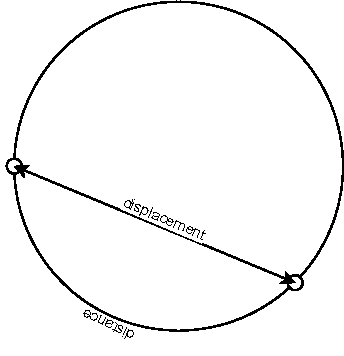
\includegraphics[width=0.4\textwidth]{displacement}
	\caption{Visualization of distance and displacement in a circle}
	\label{fig:round}
\end{figure}

We take two points on a circumference of a circle with radius r. We know from elementary math that for displacement and distance of these points holds:
\begin{equation}
	disP = r\phi
\end{equation}
\begin{equation}
	disT=2\pi{r}\phi
\end{equation}

Where we use \(\phi\) as their angular displacement in radians. When we put these equations in a relation, we get:

\begin{equation}
	\frac {disT} {disP} = 2\pi
\end{equation}

which points at sinusoidal relation between these two properties.\par
We obtain displacement between two nodes \(n_1, n_2\) by computing great circle distance between them. We will mark this displacement as \(d_{real}\). Then we will define \(d_{exp}: V^2 \rightarrow \mathbb{R_+}\) which represents the expected displacement of these nodes on a perfect circle. This value is counted from length of path between these two points that is part of the tour \(\rho\). But to use the sinusoidal relation to compute the \(d_{exp}\) we would need to know \(l(\rho)\), which is not known yet and lies somwhere in \(L\). We could be using one of the interval bounds to approximate this value, but we are going to choose different approach instead. We will approximate the relation itself to make it picewise linear. This function is clearly symetric by \(\frac {l(\rho)} {2}\) mark. In other words we get a function which meets 
\begin{equation}
d_{exp}(x) = d_{exp}(l(\rho)-x)
\end{equation}
This means we can always appoint the shorter distance by circumference to the first half of our function. The last step is to exactly express this funtion, we get
\begin{equation} d_{exp}(x)=\frac{2 min(disT, l_{max}-disT)} {\pi}
\end{equation}
where we approximated the total tour length by \(l_{max}\). Which means that this function is independent on total length of circumference - that is important fact for continuous resolution of tour roundness.\par
One more property of the edges have to be defined in order to use this function on them.
It is the location in the middle of the edge. This location, denoted as \(m(n_0, n_1), n_0, n_1 \in V\) is simplified to \(\frac {loc(n_0)+loc(n_1)} 2\). \par
Now, we can define \(d_{exp}\) for edges as well as for individual points around the tour. The expected displacement of two edges \(e_1, e_2\) will be defined by \(d_{exp}(m(e_1), m(e_2))\). For the distance around circumference of the tour from which the \(d_{exp}\) is counted we use distance traveled between \(m(e_1)\) and \(m(e_2)\) on this tour. \par
This metric has one more important feature, it can be customized to different scales of penalization for not completely round tours. We just need to add a parameter which will determine the wanted level of roundness. This envolves defining the roundness penalty function between two edges in one tour as
\vbox{%
\begin{equation}
	p(e_1, e_2) = \begin{cases}
		\frac 
			{\sigma d_{exp}(e_1, e_2)-d_{real}(e_1, e_2)}
 			{\sigma d_{exp}(e_1, e_2)}
 		& \text{if } d_{real}(e_1, e_2) < \sigma d_{exp}(e_1, e_2) \\
		0  & \text{otherwise} 
	\end{cases}
\end{equation}
}

Where \(\sigma \in [0, 1]\) parameter is called strictness and in practise define how is the perfectly round tour defined for the algorithm. To give out some examples - with values of \(\sigma\) close to zero, only edges really close to each other are penalized. We could get a tour with close to zero roundness penalty even though it won't be round at all, with shape similar to very tall oblong or rectangle. When we increase the strictness we are giving out the signal that we want more round tours but for values still further from 1 even oval tours are enough to get a perfect score. With \(\sigma=1\) every tour with not perfectly round shape is penalized.
\par
Finally we can define the average roundness penalty for whole tour \(\rho\) as:
\begin{equation}
p_{avg}(\rho) = \sum_{i=0}^{N} \sum_{j=0}^{N}\frac{p(e_i, e_j)l(e_i)l(e_j)}{l(\rho)^2}
\end{equation}
this expression should approximate the average penalty between two points randomly chosen on the tour. This means that it gets more accurate when the number of edges and length of the tour increases. This function therefore express the overall roundness of planned tour and we use its value computed with strictness set to 1 as somewhat absolute meassure of tour roundness.


\section{Original Method for Generating Closed Tours}
This is the first method that I have implemented and it follows the unoptimized version of the closed tour algorithm described in the paper from Stroobant\cite{stroobant}. The algorithm runs in two stages. \par
Where the first stage named forward routing (Section \ref{sec:forward}) aim to find candidates for a turning point. Turning point is a node \(t \in V\) to which we have found a optimal path from the origin node in terms of its weight, noted \(\rho_{s \rightarrow t}\). We use this node to get a start for the second stage of the procedure named backward routing (Section \ref{sec:back}). This stage will get path \(\rho_{t \rightarrow s}\) which will be optimal in terms of pleasentness combined with roundness penalty.\par
The pseudocode bellow describes this algorithm and is further breaked down in the following sections. The value of \(\lambda\) is defined by specific implementation or by user in the input. Its meaning is discussed in the Section \ref{sec:bestResult}. 

\begin{figure}
	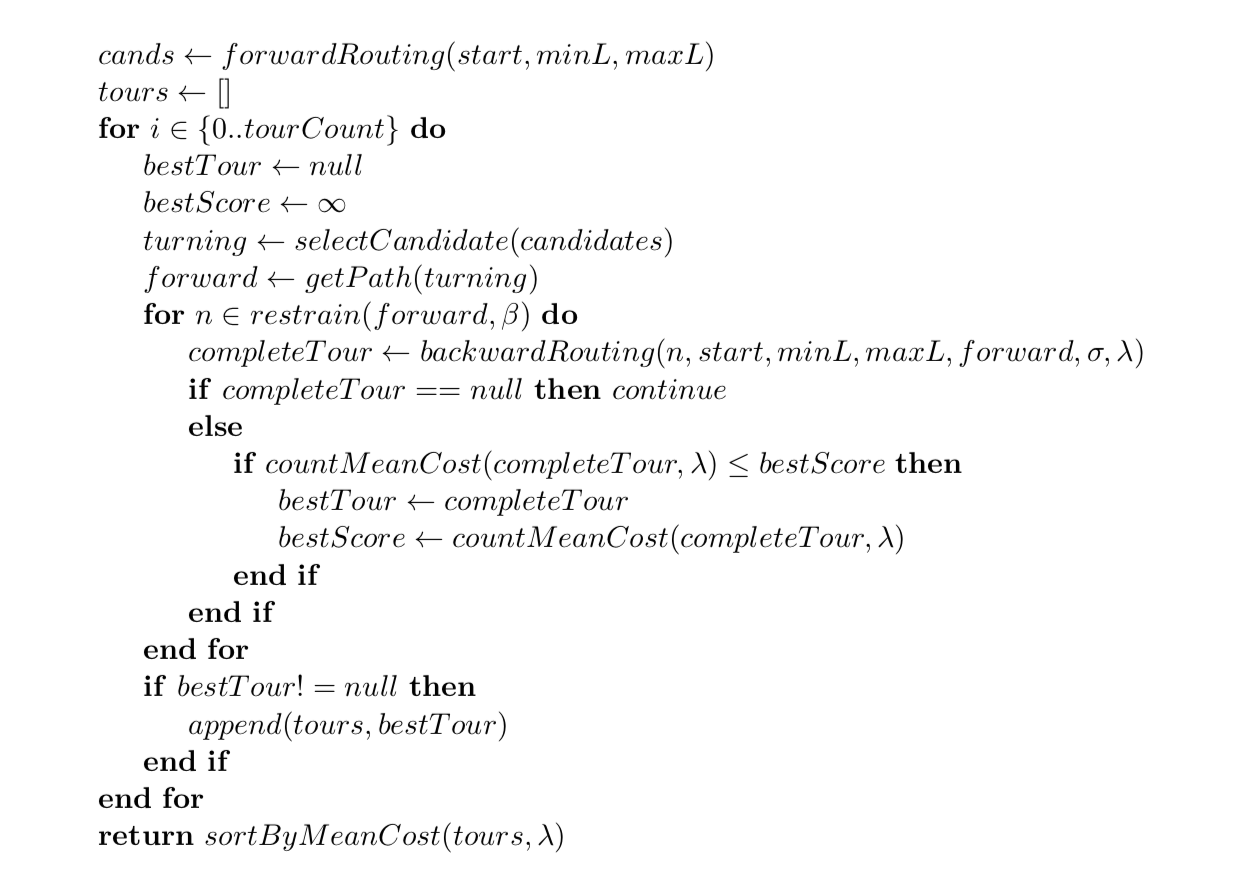
\includegraphics[width=0.9\textwidth]{pseudocode}
	\caption{Description of original algorithm}
	\label{fig:pseudocode}
\end{figure}

\begin{comment}

\begin{minipage}[t]{0.9\textwidth}
\begin{algorithmic}
\State $cands \gets forwardRouting(start, minL, maxL)$
\State $tours \gets [\textvisiblespace]$

\For {$i \in \{0..tourCount\}$}
	\State $bestTour \gets null$
	\State $bestScore \gets \infty$
	\State $turning \gets selectCandidate(candidates)$
	\State $forward \gets getPath(turning)$
	\For {$n \in restrain(forward, \beta)$}
			\State $completeTour \gets backwardRouting(n, start, minL, maxL, forward, \sigma, \lambda)$
			\If {$completeTour == null$}
    			$continue$
			\Else
    			\If {$countMeanCost(completeTour, \lambda) \leq bestScore$}
        			\State $bestTour \gets completeTour$
        			\State $bestScore \gets countMeanCost(completeTour, \lambda)$
    			\EndIf
			\EndIf
	\EndFor
	\If {$bestTour != null$}
		\State $append(tours, bestTour)$
	\EndIf
\EndFor
\State \Return $sortByMeanCost(tours, \lambda)$

\end{algorithmic}
\end{minipage}
\end{comment}


 \par


\subsection{Forward Routing} \label{sec:forward}
First stage, is meant to find all nodes which can serve as acceptable turning point for the backward search. \par 
First we have to find every candidate \(c \in V\). Base method to find all candidates is rather simple, althoug we can mount many optimalizations to it as well. For the sake of simplicity let's now consider as candidate every node \(c\) that satisfies the condition 
\begin{equation}
d_{real}(s, c) + l(\rho_{s \rightarrow c}) \in L
\end{equation}
From this specification we can derive the actual procedure to find mentioned candidates. We are going to run a graph search algorithm (in our implementation we use the Dijkstra\cite{dijkstra} graph search) that starts from the origin defined in the problem input. This search doesn't search for any specific destination node but it is hard constrained by length criterium presented earlier. Moreover, it uses the weight criterium for edge cost evaluation rather than its length. There is a fair reason for that. When candidate is found we can immidiately obtain the weight optimal path \(\rho_{s \rightarrow c}\) mentioned earlier. \par
As you can see in the pseudocode \ref{fig:pseudocode} we restrain the obtained path in some manner before sending the nodes from it further into next stage of the algorithm. Let us introduce the parameter \(\beta\). This value will determine how many points from forward route we use as turning points. Specifically we will take into account only nodes \(n\) for which stands 
\begin{equation}
d_{real}(s, n) > \beta\frac {l_{min}-\varepsilon} 2, 1 > \beta > 0
\end{equation}
For values of \(\beta\) closer to zero we get almost every node on the forward path and we use them as a turning point for backward routing. Values close to one will drop the whole first half of the path \(\rho_{s \rightarrow c}\) and we select the rest as a suitable turning points.

\subsection{Backward Routing} \label{sec:back}
I am going to assume we have just one turning point \(t\) linked with proper forward path \(\rho_{s \rightarrow t}\) found in first stage. Now we have to find suitable path back from this turning point.\par
This path \(\rho_{t \rightarrow s}\) has to follow the condition 
\begin{equation}
l(\rho_{s \rightarrow t}) + l(\rho_{t \rightarrow s}) \in L
\end{equation}
Moreover, it should optimalize the weight \(w\) in combination with tour penalty \(p\). To obtain such back path, we launch yet another graph search, now from \(t\). This search is aimed toward \(s\), constrained by \(L\). On top of that, we need to include geospatial diversity against forward path to the overall cost \(c\) of every edge \(e\) expanded by this search. We can get a number expressing this diversity by computing the roundness penalty against every edge in the forward path, normalized by tour length.
\begin{equation}
p(e, \rho_{s \rightarrow t}) = \frac {2 \lambda} {l_{max}} \sum_{e' \in \rho_{s \rightarrow t}} {p(e, e') l(e) l(e')}
\end{equation}
 We approximated the tour length (which is not known in the time of computation) as a upper bound on the tour length. Next, we combine this value together with edge weight to get a expression describing an overall cost of an edge.
\begin{equation}
c(e) = w(e) + p(e, \rho_{s \rightarrow t})
\end{equation}
This overall cost fulfills every property which we defined in the problem definition. It makes harder to revisit the same edge on the path back. Level of this resistance is proportional to user defined parameter \(\lambda\). \par But note that it never straight out ban the revisiting. And this is also an important feature which has a great positive effect on solvability. Such restriction would effectively exclude from planning every part of the graph that is connected by one edge only to the rest of the network. And that would make the search completely unusable in some areas. \par
Also, this penalization does not work with edges only, user get to define \(\sigma\) to choose what is the actual size of surroundings around forward path, where will be backward path search penalized. This is also a neat feature, beacuse it allows user to prefer perfect round tours or on the other side turn off this penalization all together.\par
The search could end by two ways. The first is when there is no path \(\rho_{t \rightarrow s}\) that would fullfil the length criterium. In that case we simply have to move to another turning point and repeat the process.\par 
The second way is when the search reaches the origin point. In this moment we got two paths \(\rho_{s \rightarrow t}\) and \(\rho_{t \rightarrow s}\) by their combination we got a valid solution to our problem. \par However, this is only a solution to the smaller subproblem dependent on chosen forward path. As we can see in the pseudocode at the start of this chapter we should search from multiple turning points that are part of different forward paths to get a bigger chance to found the global optima of the problem instance defined by the specific input combination. \par

\subsection{Selecting the Best Result} \label{sec:bestResult}
The input to this final stage of the algorithm is multiple tours, which meet the hard criteria defined by input parameters. Next up we need to restrict this set or at least sort it, to get the most promising tours from it.\par
In order to achieve this we define the property which we are trying to optimize as:
\begin{equation}
c_{avg}(\rho) = w_{avg}(\rho) + \lambda p_{avg}(\rho)
\end{equation}
Where \(c_{avg}\) represents overall mean cost of the tour, \(w_{avg}\) mean pleasentness and \(p_{avg}\) stands for mean roundness of the tour as described earlier. \par 
The \(\lambda\) parameter in this expression represents the emphasis on tour roundness in comparison to the tour pleaseantness. It is easy to spot by plain sight that \(\lambda\) close to zero will not take roundness into account much, the main component of the final cost will be the cost of individual edges in the walk only. However greater values of \(\lambda\) can lead to another extreme where penalties for roundness overshadows edge cost and algorithm searches for round tour with zero roundness penalty rather than optimalizing cost of the edges. This parameter will allow to use more flexible evaluation based on user preferences or local conditions. \par


\subsection{Extension to Point-to-Point Tours} \label{sec:ext}
As is mentioned in the introduction, the recreational cycling is not restricted to the closed tours and so should not be our algorithm. But to achieve this there are two modifications that have to be done on the original algorithm. \par
This first one is to extend the forward routing routine to work with the destination point \(g\). In the point-to-point version, we aim for this node and therefore we have to restict the forward routing search by:
\begin{equation}
d_{real}(g, c) + l(\rho_{s \rightarrow c}) \in L
\end{equation}
\par
The second modification concerns the computation of roundness. We defined the roundness which is not dependent on the total length of the resulting tour as far as we always plug in the shorter distance around the supposed circumference. This shorter distance was computed from the path length between two edges \(disT\) or the \(l_{max}-disT\). It is clear that we cannot use the second expression anymore as it would falsely assign a very small displacment to two edges at the opposite sides of point-to-point tour. \par 
What we will do instead is that we will always insert the \(disT\) value into the formula. Together with this we will naturally restrict the edges too far away from actual edge from the set against which its penalty is computed. This has a straightforward logic as this edges shouldn't be a concern for our user, because point-to-point tours are not restricted to perfect half circles only. For example, imagine tour which curls back and forth multiple times between the origin and destination point. This tour is still completely suitable for our purpose as it does not visit any region twice. Roundness penalty defined like this could result in a curly path where it takes care of minimal number of returns and traveling by the same segments of the road. The bigger the strictness, the biger is the diameter of these curls.

\section{Modified Version of Generating Tours} \label{sec:modification}
When running the original version version of the algorithm I noticed that there are two key factors in the performance of the algorithm. The factor which has the biggest impact on the solution quality is the selection of the candidate node and forward path associated with it. The factor which has the biggest impact on the running time of the algorithm is the backward routing stage and how many individual backward searches runs in this stage. Therefore I decided to modify the original algorithm and address these two issues in this modification.\par
The fact we have to realize is that there excessive number of candidates in the set grouped closely together. And the smaller the distance between two candidates the higher the probablity that the optimal paths from the origin point share most of the segments with only small diversion at the end. This has the consequence of using many turning points multiple times in the backward routing stage. These searches will also result in a tours which are similar or outright identical with one another. Therefore even a lot of used candidates in the same area with high unpleasantness won't find the optimal solution and on top of that it is a complete waste of computational resources.  \par
The first thing I have changed is that I implemented a mechanism which will run one or multiple filters over the candidate set to remove the ones with the smallest potencial. These filteres and their working is the main topic of the next section \ref{sec:filter}. \par
The second step I took was to completely abandon the multiple backward searches from the nodes on the path from origin to the selected candidate technique. This step saves a computational resources in a very notable way. Moreover, with a smart choice of filters and selecting mechanism from the candidate set, there almost isn't drop in planned tours quality. 


\subsection{Filtering and Selecting Candidates} \label{sec:filter}
From now on I am working with set of candidates obtained in the first stage of the algorithm. \par 

The most simple approach to the selection would be to simply select from this set at random but that has obvious impact on the result quality. Instead, we could easily point the selecting mechanism to the candidate set that has much better probability to result in close to optimal set of solutions. One of the options is to sort the candidates by best mean cost of their forward paths. These paths have higher probability to be included in the optimal solution.\par

Another technique is to take into account the geographic location of picked candidates. We can favor picking sets of turning points which are most geospatially diverse. This has several benefits. For one it makes higher the chance to find the optimal solution to the problem instance as the algorithm will search through much bigger space. And for the second this technique is also benefical for the end user. It naturally yields geospatial diverse sets of solutions. And we know these results are the most attractive for people that use external suggestions for recreational tours as it bring more distinctive choices for the user to choose from.\par

But by far the most effective technique is to filter out the most unpromising candidates all together. I am going to describe multiple filters in this section that aim to find and remove such nodes.


\begin{figure}[!tbp]
  \centering
  \subfloat[Removing dead ends]{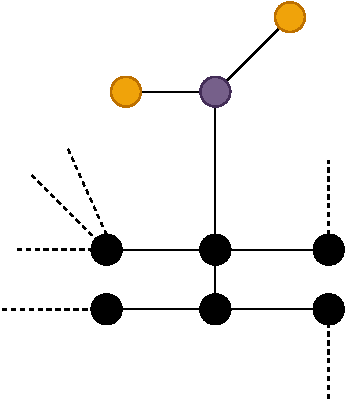
\includegraphics[width=0.4\textwidth]{deadEnds}\label{fig:f1}}
  \hfill
  \subfloat[Node contraction]{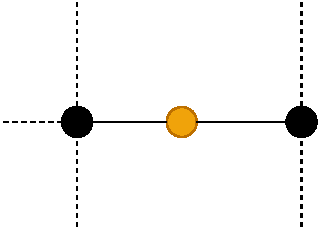
\includegraphics[width=0.4\textwidth]{contracted}\label{fig:f2}}
  \caption{Examples of candidate filtering}
\end{figure}

\subsubsection{Dead End Filter}
The first filter is the one most convenient method to avoid unnecessary returns along the planned tour. The idea behind this filter is to remove all candidates that would, if picked, result in tours that have in the immediate surroundings of the turning point one or more recurring segments. Part of one such tour is displayed in the \ref{fig:return}. Aside from this positive effect, there is also one tradeoff that has to be done. In this problem we take into account the hard constraint on the total length of the tour determined by interval \(L\). By limiting the candidate set you can encounter cases where every tour found is too short and this small segment of return around turning point would add up the length needed in order to get above the lower bound of the interval. \par
The filtering itself run in multiple steps. The first one will remove all the nodes that have only one neighbour in the graph. Each next step will extend this rule to ignore already removed candidates as neighbours. Both steps are pictured in the \ref{fig:f1} where black nodes show candidate nodes, orange ones show nodes removed in the first step and the purple one is the node removed in the next step. 

\begin{figure}
	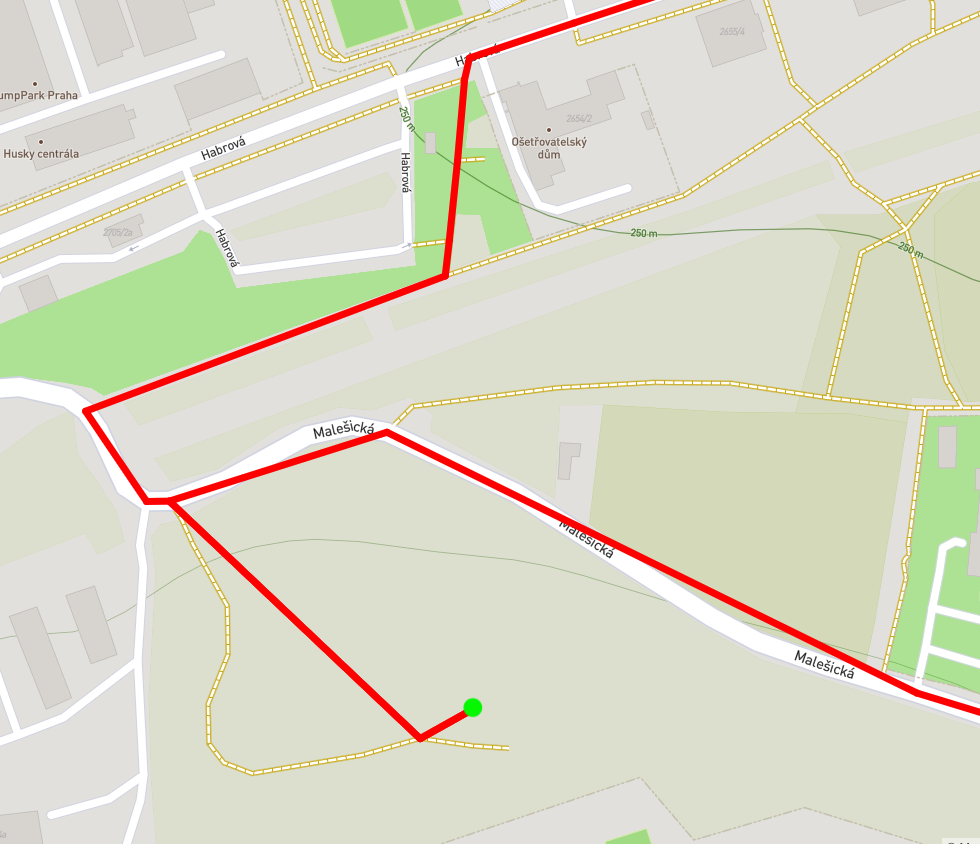
\includegraphics[width=0.7\textwidth]{return.png}
	\caption{Tour with return from turning point located in one of dead ends of the graph}
	\label{fig:return}
\end{figure}

\subsubsection{Contraction Node Filter} 
Second filter which we proposed and implemented is again intended to lower the total number of candidates and higher their mean distance. It achieves this by removing candidates from the set that are surrounded by exactly two other acceptable candidates. \par
Let us imagine the case of one simple edge between two points (say \(f\) and \(n\)) with single via node \(v\) in the middle. The via point is of degree 2 and the nodes at the start and end of the edge are of degree 2 or more. Moreover all three nodes are in the candidate set. We choose the point \(v\) as our turning point. It is easy to prove that the path found to this node is (except the very last segment) the same as path found to either \(f\) or \(n\). To revolve around specific case let's think of \(f\). The best path back from \(v\) goes either through \(n\) or \(f\) again. The latter case results in path which is very similar to the one we would get if we chose the node \(f\) itself, except it has the return around turning point similar to the one described in previous section. The former would result in nice smooth tour. But if this is the case, we would get exactly the same result choosing \(f\) or \(n\) as turning point. Therefor we can neglect that via node with ease. \par
One of these candidates to be removed is pictured in orange in \ref{fig:f2}. \par
On the top of positive effects on the candidate set mentioned in the opening paragraph of this section we get the same tradeoff as in the previous case with this filter. It prunes the solution space from many solutions that contains returns. As mentioned previously this is beneficial to the smoothness of found solutions but also some quite acceptable solutions with returns will be inevitably pruned.

\subsubsection{Path to Distance Ratio Filter}
The last from these filters that I have implemented works by comparing the length of the minimal cost path to each candidate found in the forward routing stage and great circle distance to the destination node. It filters candidates with extreme values of this ratio. \par 
The reasoning behind this approach is that such an approach greatly increases the number of round tours in the solution set without the need to count an excessive number of tours to find these "pretty" tours. Just imagine how this candidate with extremely low or high ratio looks like. These are in most cases nodes that are extremely close to origin or destination node of the request. And by choosing such candidates we will plan either extremely short path to or from this candidate to the destination node. Both of these cases are problematic, as we count the roundness penalty against forward route when planning backward route. The first case results in a very small penalty for each edge on backward route, which could lead to tour revisiting the same region multiple times because there is no penalization for it. And in the second mentioned case there is simply no space for a tour to take an acceptable shape by planning a short backward route with roundness penalty. The filter is therefore proposed to let the developer specify the upper and lower bound ratio. Only nodes whose shortest path and distance to destination satisfy this ratio are passed to the next stage.


\chapter{Implementation}
To demonstrate algorithms described above I implemented them in a Java 8 application using Open Source libraries. This part of the project and its dependencies are managed in Maven. \par The individual components and architecture of this implementation are further discussed in Section \ref{sec:solutionImpl}. \par This application is furthermore wrapped as a webservice exposing REST API.\cite{rest} Every application can submit parameterized requests for route planning. The best routes are then returned as a response. Inner structure and endpoints of this service are broken down in Section \ref{sec:service}. \par On top of that, I build a simple web client in Javascript which can consume the web service and make the process easier for the user. It also provides visualizations and debug data. A brief description of this client is located in Section \ref{sec:client}.\par There is a public version of both client and server codes available in the root repository for this thesis.\cite{git} Instructions on how to use them are at the end of this chapter.


\section{Algorithm Implementation} \label{sec:solutionImpl}
\begin{figure}
	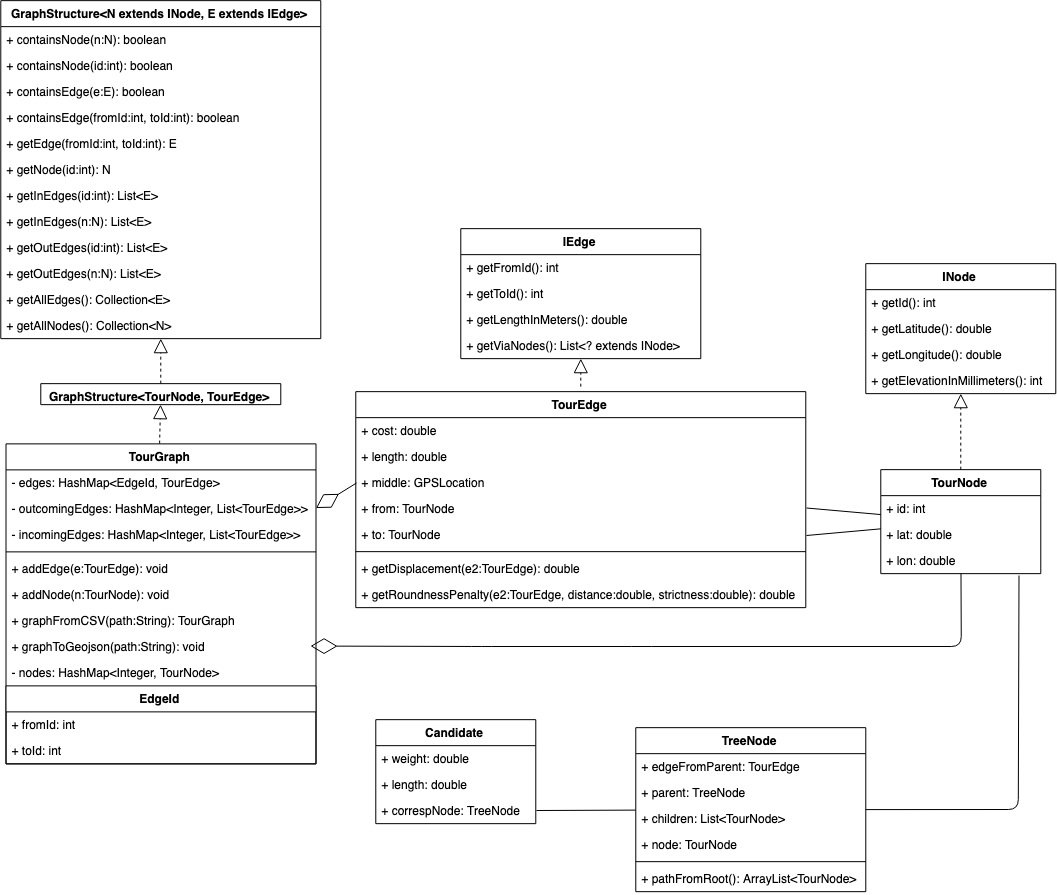
\includegraphics[width=0.8\textwidth]{graph.png}
	\caption{Graph objects structure}
	\label{fig:coreGraph}
\end{figure}

For the representation of the graph and its individual features I chose to implement interfaces from \codeword{base-structures} library provided to me by the Umotional company.\footnote{Residing at \url{https://umotional.com/}.} The interfaces I used (specifically \codeword{INode}, \codeword{IEdge} and \codeword{GraphStructure}) encapsulate the basic methods that should be available on the graph objects in order to make it more convenient to work with them. Implementations of all these interfaces I used are available in \codeword{model} package. The second great motivation for this approach was the ability of other libraries to work with these interfaces. \par
The graph loaded into the \codeword{TourGraph} object should be stored in the CSV file. This CSV file does specify every edge in the graph. Edges are specified in terms of IDs of end nodes, their GPS location, edge length, and cycling inconvenience. Several examples of these files can be found in the repository\cite{git}. \par
The original graph, which was used as a base for the service as well as in the experiments, was once again provided by the Umotional.\footnote{Residing at \url{https://umotional.com/}.} It is a variation of a graph downloaded from the Geofabrik server\footnote{Available from \url{http://download.geofabrik.de/}.}, cropped to Prague and its closest surroundings. Graphs on this server are extracted from OpenStreetMap project data and cleaned from all superfluous metadata. The data was further processed by its tools to make it more suited for bicycle trips planning, which means removing highspeed roads, interpolating long edges, etc. \par


\begin{figure}
	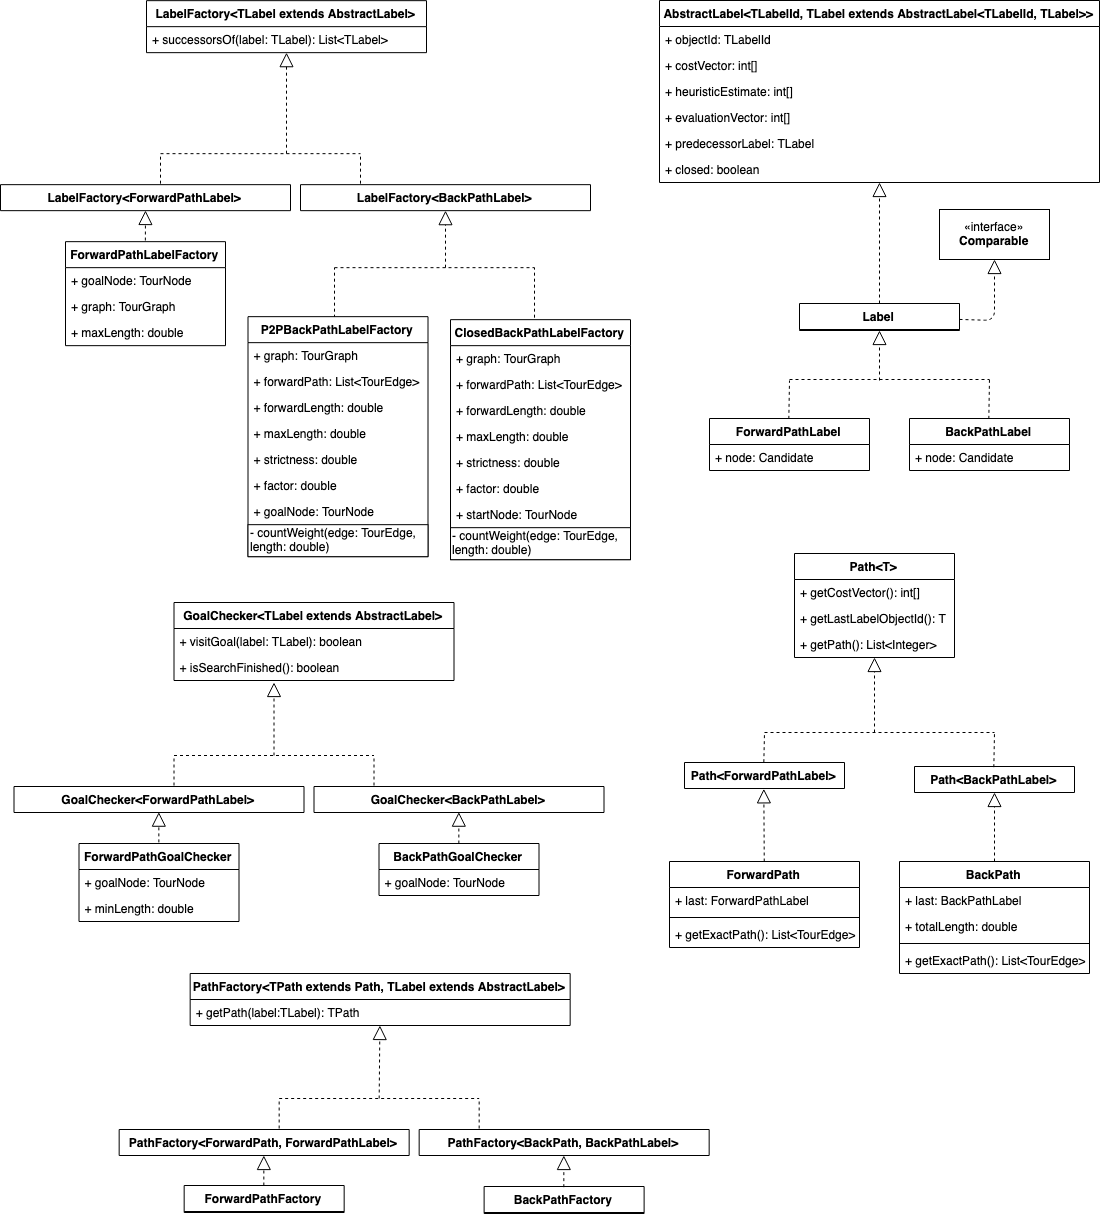
\includegraphics[width=0.6\textwidth]{search.png}
	\caption{Structure of objects used in searches}
	\label{fig:corePlan}
\end{figure}

To implement forward and backward routing I chose to use yet another open source library from Umotional company.\footnotemark[\value{footnote}] It is \codeword{core-planning-algorithms}. The library provides a functional framework to implement almost any graph search algorithm. It creates a higher level of abstraction with the help of several general interfaces that encapsulates the basic actors and methods present in every graph search algorithm. Everyone can then create their own implementation of these interfaces. Moreover, this library already provides the implementation of basic well-known algorithms as is, for example, Dijkstra\cite{dijkstra} or A*\cite{astar}. I used this implementation of Dijkstra, in combination with custom made classes pictured in Figure \ref{fig:corePlan}. All code concerning these searches is located in the packages \codeword{forwardpath} and \codeword{backpath}.\par

The core class of the implementation is \codeword{PlannerService}. It plays main role in both standalone application run locally and web service. It is outlined together with its dependencies in Figure \ref{fig:coreService}. This static class manages all backend logic. At the start of the application it loads graph, creates an index over all nodes, creates complementary objects as are \codeword{CandidateFinder} or \codeword{BackpathFinder} and more. After this boot-up phase, it is ready to accept requests for planning. \par

\begin{figure}
	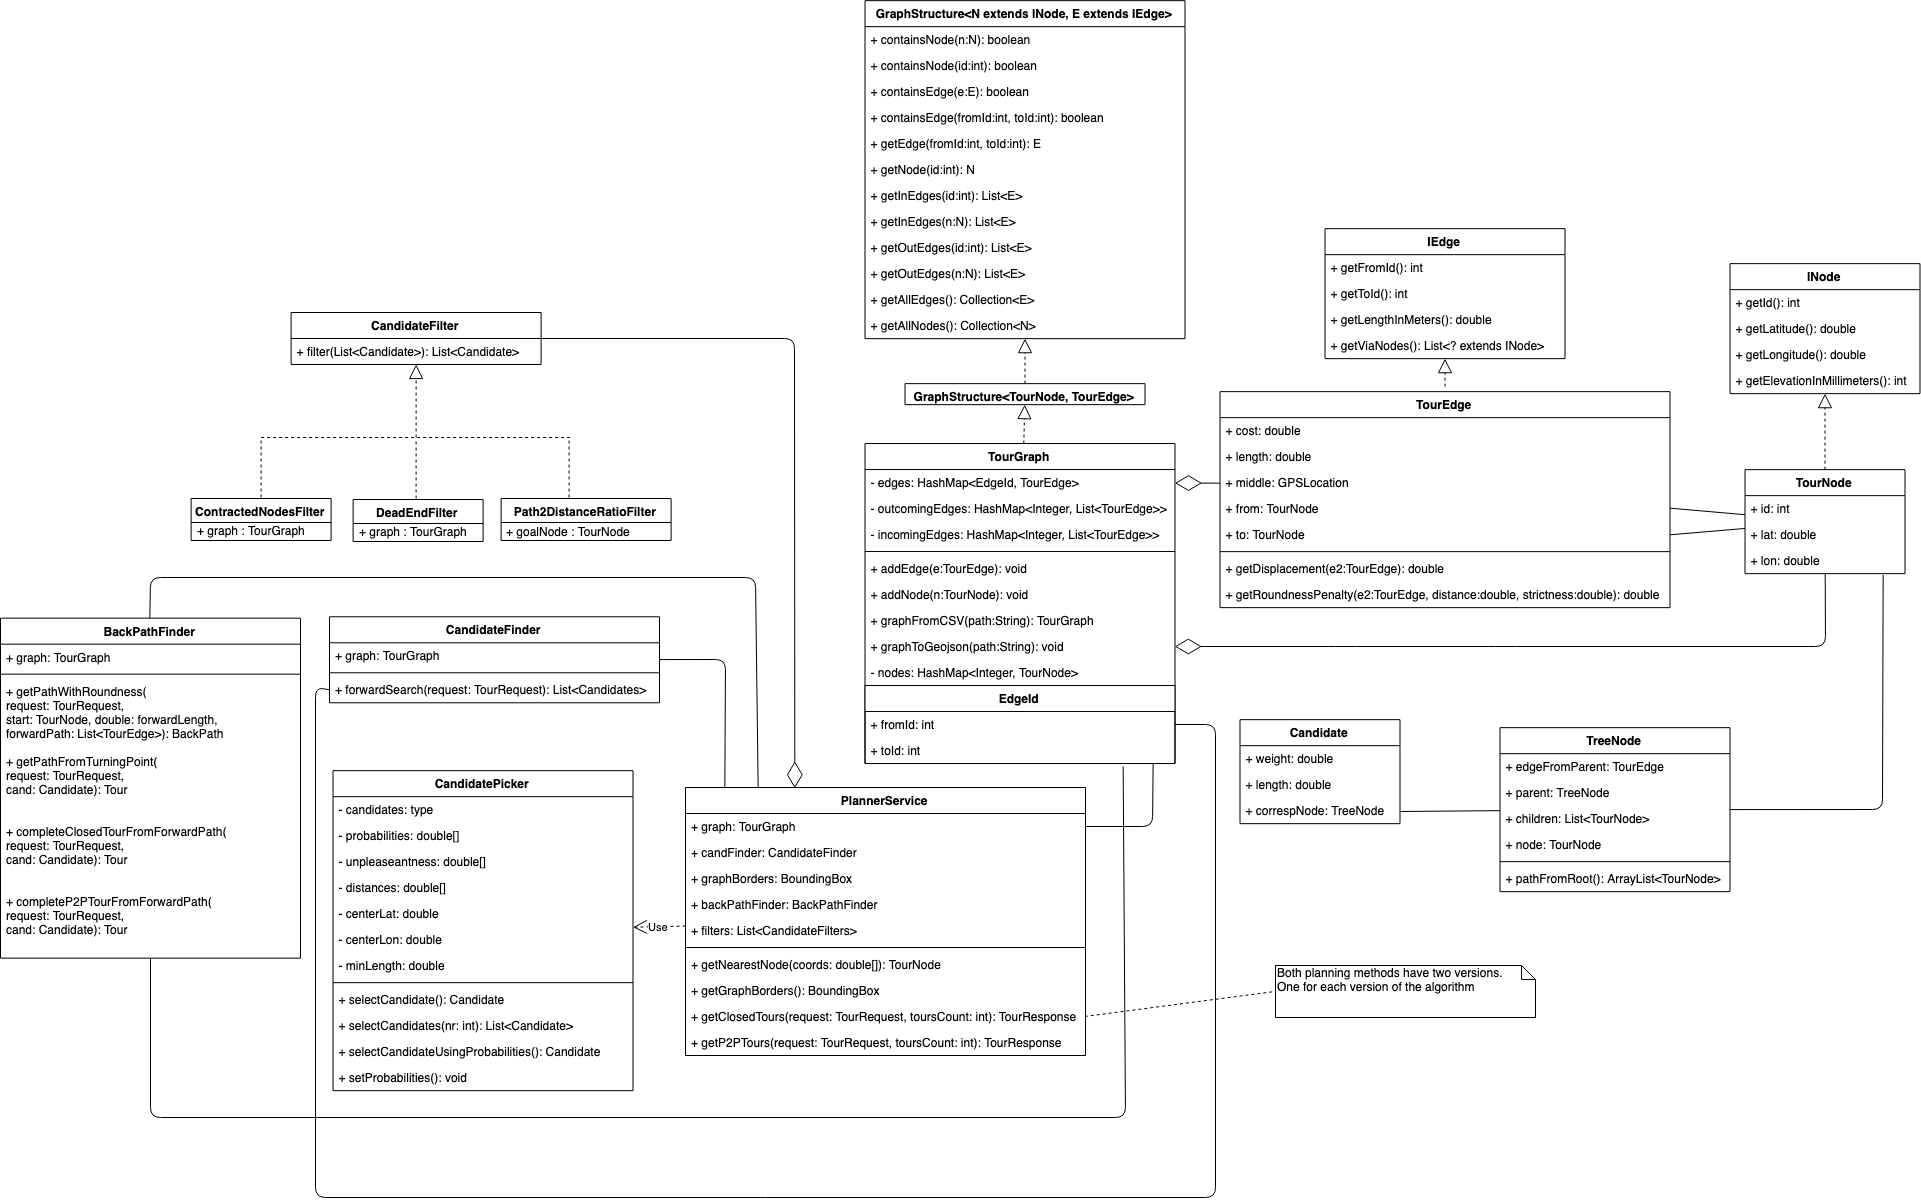
\includegraphics[width=0.8\textwidth]{service.png}
	\caption{Service objects structure}
	\label{fig:coreService}
\end{figure}

The last important pieces of code are to be found in the \codeword{utils} package. This package provides methods that are not specific to one of the classes or process but are used extensively throughout the whole codebase. It includes classes as \codeword{IOUtils} that is taking care of visualization and dumping to the local files. Or \codeword{TourUtils} where are the computations of distances between objects, length of the paths, etc.



\section{Web Service} \label{sec:service}
I implemented the API using Jersey Framework \footnote{Avaiable from \url{https://jersey.github.io}.} in combination with standart Java Servlet API. This framework makes creating RESTful APIs\cite{rest} much easier. It enables using of specific annotations, package specification, custom request filters and more. \par
Classes created with the help of the framework are located in the \codeword{api} package. These clases defines the endpoints described in Section \ref{sec:api} and handles traffic that is comming through them. They are connected to the \codeword{PlannerService} class that is created at the start of the web service and that is managing the actual computations to provide adequate response to the planning requests. \par
On top of that Jersey gives out the Jersey Maven plugin that is used for deployment of this service. 

\subsection{API} \label{sec:api}
There are several methods that can be invoked via web call to relevant endpoint. Each method accepts data in form of querry parameters that are passed on to the service implementation as arguments.

\begin{figure}[H]
	
\includegraphics[width=0.9\textwidth]{communication}
	\caption{Simple schema of implementation part of this project.}
\end{figure}

\subsubsection{Closed Tours and P2P Tours Endpoint
   \\ {\normalfont{\textcolor{black!70}{\texttt{/closed}}}}
   \\ {\normalfont{\textcolor{black!70}{\texttt{/p2p}}}}
   }
   These are the core endpoints of the service that are used for planning of the recreational routes, both of them are connected to the \codeword{PlannerService} class.\par The nature of the tour is given by the choice of the endpoint to call. Both of them share the same query parameters that are defined in the Chapter \ref{chap:solution}. These parameters are parsed to the \codeword{TourRequest} object. They provide \codeword{TourResponse} object as an answer to the call. Structure of both objects is depicted in Figure \ref{fig:apiParam} \par
   If the request is poorly specified the service will answer with the HTTP code 400. This can sign, for example, non-existing node as origin or destination parameter. When no tour is found within the current input the service returns HTTP code 404.

   	\begin{minipage}[t]{1\textwidth}
		Available parameters:
		\begin{itemize}
			\item start - ID of origin
			\item goal - ID of destination
  			\item minLength - \(l_{min}\)
  			\item maxLength - \(l_{max}\)
  			\item strict - \(\sigma\)
  			\item factor - \(\lambda\)
  			\item count - Size of candidate subset
  			\item method - which algorithm to use (1 - modified, 0 - original)
		\end{itemize}
	\end{minipage}

   


\begin{figure}
	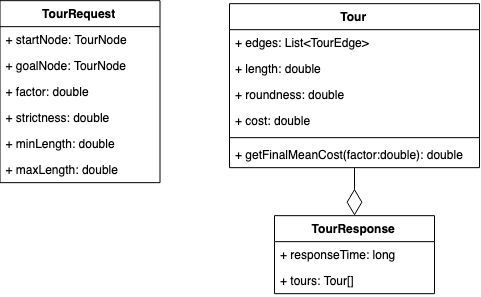
\includegraphics[width=0.7\textwidth]{api.png}
	\caption{Planning request and response objects}
	\label{fig:apiParam}
\end{figure}

\subsubsection{Nearest Node Endpoint
   \\ {\normalfont{\textcolor{black!70}{\texttt{/map}}}}
   }
The core functionality of the service i.e. the planning of the tours described above is designed to accept just a node ID as a part of the TourRequest. Although this makes the communication easier from development side of view it is not very convenient for the end user. Therefor this endpoint is available - to translate pair of coordinates into the ID of the nearest node in the graph. The most obvious use case for this endpoint which is also used in my client implementation is to let the user click at some point in the map and obtain the nearest node ID to use in the actual request. \par
The inner working of this method is provided by KDTree object. This object is slightly edited version of KDTree from \codeword{javaml} library.\footnote{Avaiable from \url{http://java-ml.sourceforge.net/}.} This static object is created together with the service and filled up with every node in used graph. We choose object dimension in the size of two as our coordinates has two components also. This allow us to use the basic great circle distance of two points as the resolver function when searching through the KDTree. In the end this approach greatly outspeed sorting or filtering nodes in simple list, but with slightly worse space complexity.

\begin{minipage}[t]{1\textwidth}
Available parameters:
\begin{itemize}
  \item lon - longitude of location to map
  \item lat - latitude of location to map
\end{itemize}
\end{minipage}

\subsubsection{Graph Borders Endpoint
   \\ {\normalfont{\textcolor{black!70}{\texttt{/border}}}}
   }
This is just a simple enpoint that serves to either visualize the graph borders in the client appliccation or to restrict the requests entered by user to fit currentlly loaded graph.  It returns the greater bouunding box of the graph in GeoJson format. 


\section{Client Implementation} \label{sec:client}
This section describes individual parts of the web client located in the \codeword{frontend} folder. The client was implemented in the mix of HTML, CSS and Javascript. \par

\subsection{User Interface}
The user interface provides a handy way to specify every parameter of the request. After the page is loaded, the client calls the Graph Borders endpoint and visualizes the response; this shows the user the part of the map that supports the tour planning. This area is defined by a black rectangle as you can see in the \ref{fig:UI}.\par The most significant part of the user interface is a request console that you can find on the left side. This console allows you to set every parameter of the \codeword{TourRequest}. Moreover, it offers a switch at the bottom with which you can control if the server returns tours planned by the first or the second method as described in Chapter \ref{chap:solution}. Entering these parameters is pretty self-explanatory. \par The only thing worth of closer explanation is the input of both the origin and the destination node. At the top of the console there is a control which switches the mode of the search from closed tours to point-to-point tours and back. The nodes themselves are then chosen by a user click into the map. This click invokes a call to the backend, which gives back to the client the GPS location mapped to the nearest node. Following this exchange, the client fills in the node ID to the input and puts a marker into the map for an easier orientation. After submitting the whole form, the client creates a request with all the inputs used as a query parameter.

\begin{figure}
	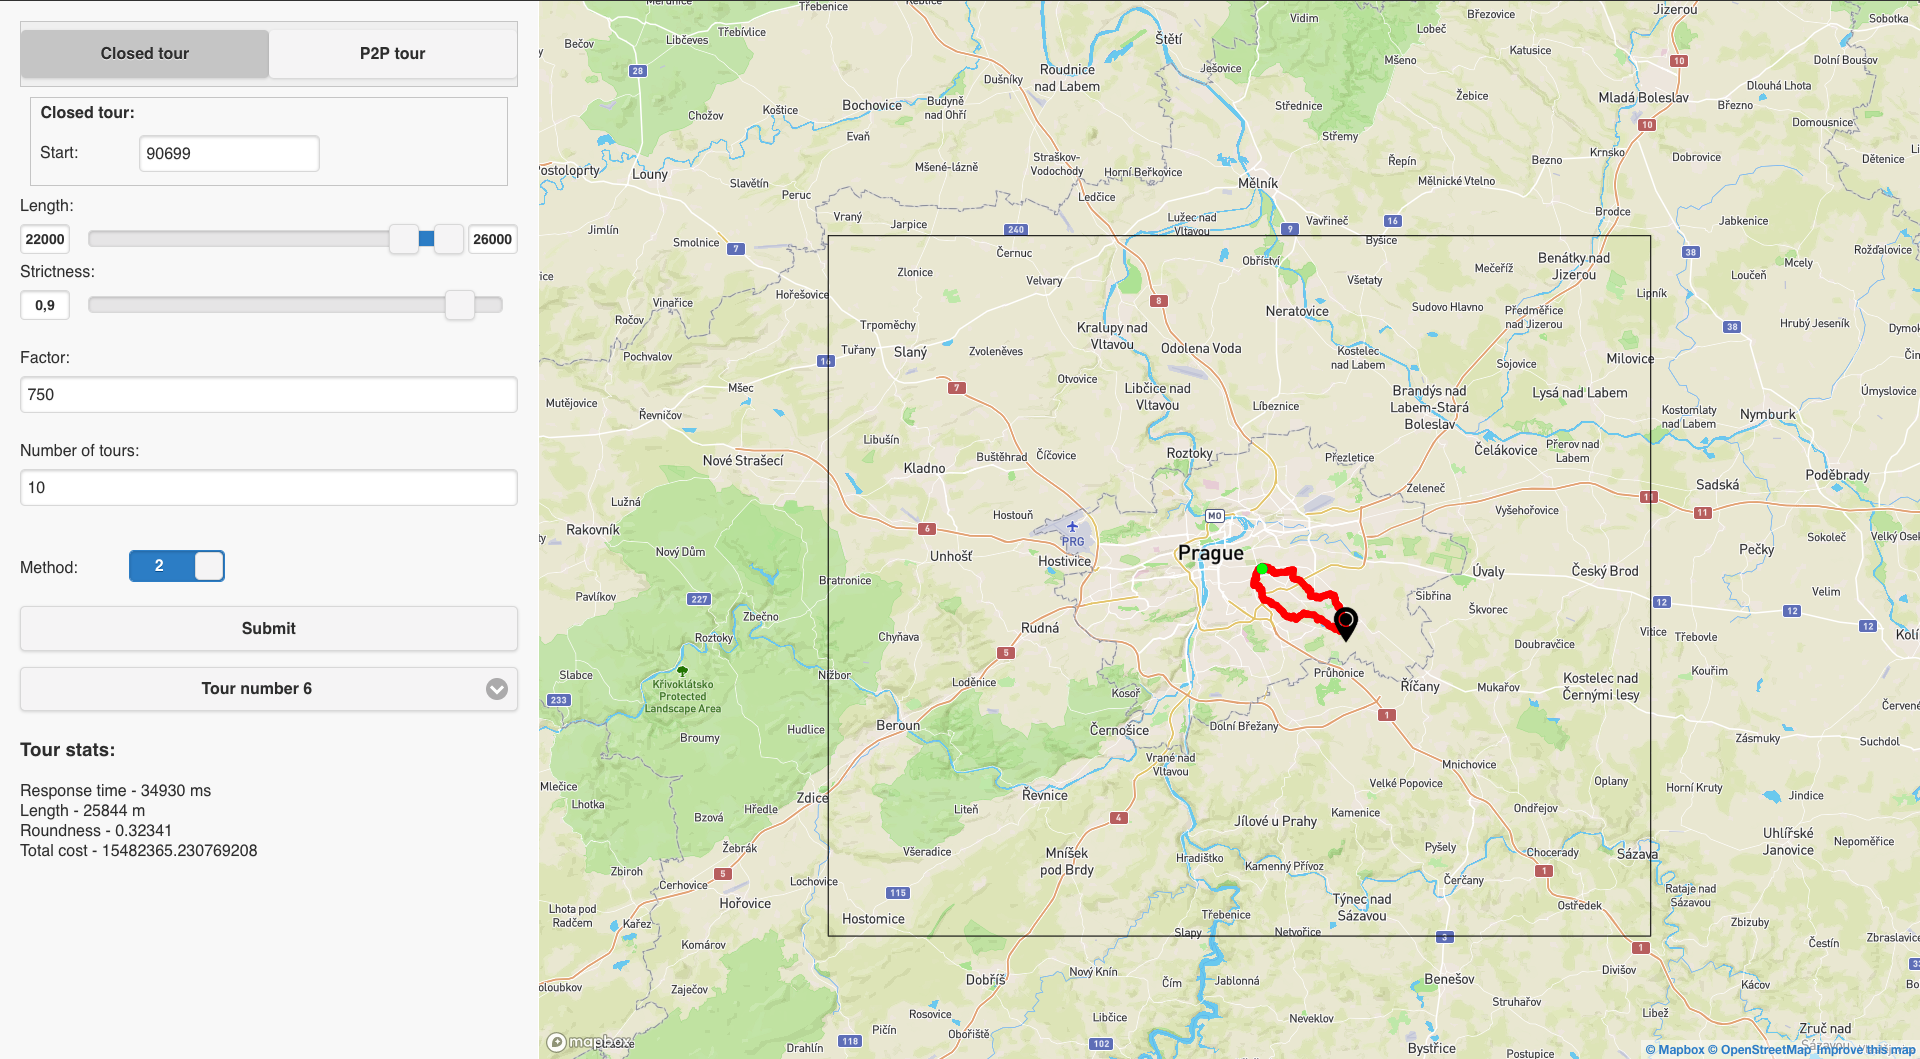
\includegraphics[width=0.9\textwidth]{UI}
	\caption{UI of the web client}
	\label{fig:UI}
\end{figure}

\subsection{Tour visualization}
When the server returns the \codeword{TourResponse} object to the client it loads all the returned \codeword{Tour} objects into the page. You can switch between them by list selector located in the lower left area. The debugging information about tour is always provided right below this selector. \par
The visualization of the tour shows three important things. The first one is the tour itself laid over the real world map. Second is the original candidate of this tour marked by a green dot. And the third one is a used turning point marked by a blue dot. In the modifed version of the algorithm these two points are identical. Example of such visualization can be found in Figure \ref{fig:vis}.

\begin{figure}
	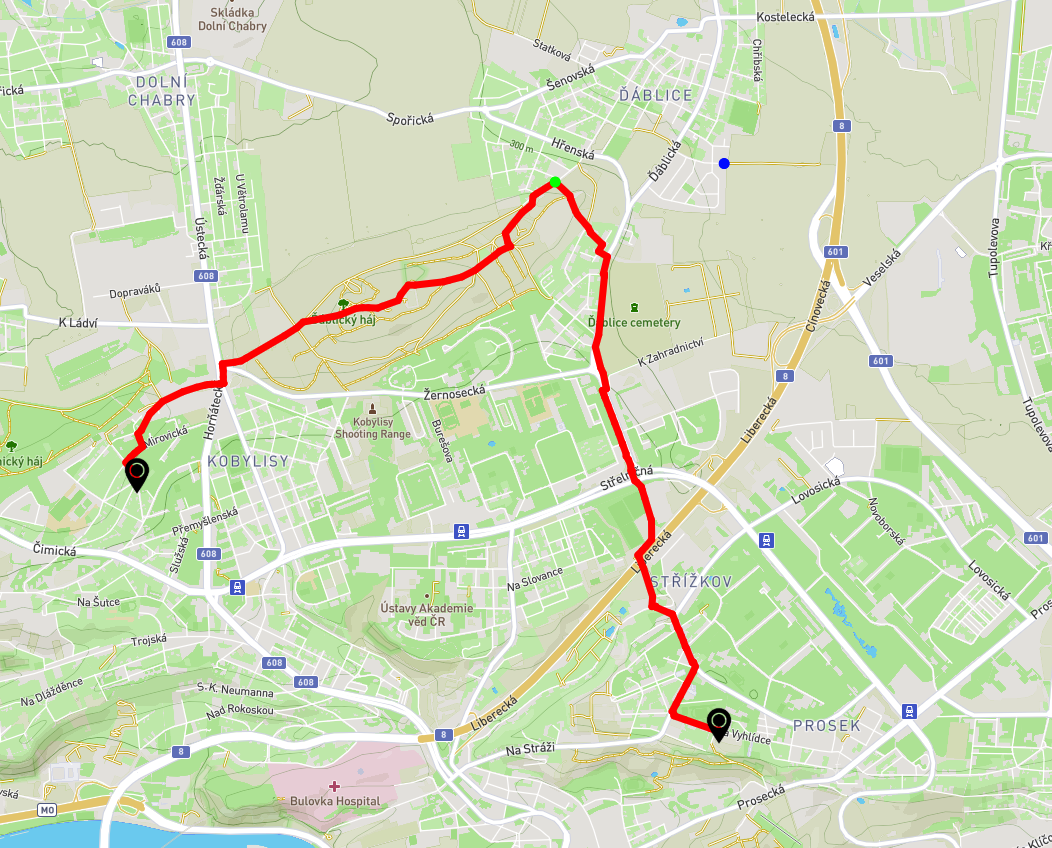
\includegraphics[width=0.9\textwidth]{plannedTour}
	\caption{Tour visualized in the web client}
	\label{fig:vis}
\end{figure}


\section{How to Run}
The code available in the repository is entirely ready to be run locally as either Java application or web service. The Java application does accommodate all experiments from Chapter \ref{chap:performance} the web service follows the definition outlined in Section \ref{sec:service}. \par

\subsection{Web Service and Client}
You can run it easily as web server by using the Maven Jetty plugin. It takes just one command on the project directory level. \codeword{mvn clean jetty:run} will wrap the whole project and deploy its server instance. After quick boot up, the server is ready to accept requests on endpoints described in \ref{sec:service}, which are to be found on the port 8080. There is a default setup in place that uses an example graph representing a smaller part of Prague, which is stored in resources. You can overwrite the configuration in PlannerService source file where you can even specify one of your CSV files if it follows the same format as CSV files attached to the project. If you wish to deploy the service in any other way you can use \codeword{mvn compile war:war} to obtain the WAR file with it.
The client is set up to work with the server deployed through the Jetty plugin. If you simply open \codeword{index.html} file from the frontend folder it will interact with it as described. To use the frontend with a remote server on a different location, change the \codeword{address} parameter at the top of the \codeword{script.js} file to its location. \par
As a time of writing there is also a functioning demo available to try at the address \url{http://test.umotional.net/tour-planner-frontend/}.
\subsection{Experiments}
If you wish to run the experiments specified in chapter \ref{chap:performance} you can use command \codeword{mvn clean install} to get a JAR file with their implementation. This JAR file will prompt you for an arguments specifying which experiments will be conducted and what is the path to the base graph. But note that to run this experiments on other graph than \codeword{prague.csv}(included in the attachements) you have to change the IDs of tested nodes in the class \codeword{ExperimentMain}. \par




\chapter{Evaluation} \label{chap:performance}
In this chapter, I focused on the evaluation of proposed solutions and their implementation. There are three distinctive experiments. Each experiment is testing exactly one input parameter. In each experiment, multiple requests are evaluated by both versions of the algorithm - the original and the modified one. The combination of experiments will help us understand the differences between the two versions and their performance in different environments.\par All experiments were conducted on the closed tour planning, the main reason being that the roundness experiments (Section \ref{sec:testRound}) are practically non-telling in the point-to-point tours. But there should be no major deviations from the results of other experiments if we use the point-to-point planning as the modifications I described in Section \ref{sec:ext} have no practical impact on properties tested in these experiments. \par The graph which I have used for all experiments is a graph of Prague and its surroundings obtained by the same procedure as described in Section \ref{sec:solutionImpl}. This graph features 205130 nodes and 559398 edges in between them. \par The most crucial factor influencing the algorithm performance is the choice of origin and destination of the tour. The quality of results can vary from place to place depending on the road network - its density, the length of the nearby segments, the average degree of nearby junctions and so on. And there are of course areas where it is not possible to find even one tour with the chosen parameters. To mitigate these effects, we chose ten distinctive nodes across the whole graph and run identical request on every one of them. These nodes were used as origin locations in each one of these experiments. The results you can see in diagrams are the averaged values from these requests. This helps us to relate the experiments to each other as they are undistorted by this factor.\par All experiments were conducted on a machine with four cores of Intel(R) Core(TM) i7-7700 CPU @ 3.60GHz. The experiments were requesting around 19 GB of vitual memory, the amount of resident memory did not exceeded 512MB. \par

\section{Selected Candidates}
As you can recall from Chapter \ref{chap:solution}, which was describing the solution, after the forward routing phase comes the part where we pick some smaller subset of candidates from all of the acceptable nodes. Then we use this subset in a following backward search.\par The first experiment is meant to observe and describe the relationship between the performance of the algorithm and the total size of this subset. We are going to compare the performance of both described methods over identical instances of the problem. The performance is measured by two metrics - computation time and mean cost of the best solution. \par 

\begin{minipage}[t]{0.9\textwidth}
	The setup of this experiment:
	\begin{itemize}
  		\item Minimal length: 16000m
  		\item Maximal length: 18000m
  		\item Factor: 450
  		\item Strictness: 0.9
	\end{itemize}
\end{minipage}
\vspace{20px}


\begin{figure}
	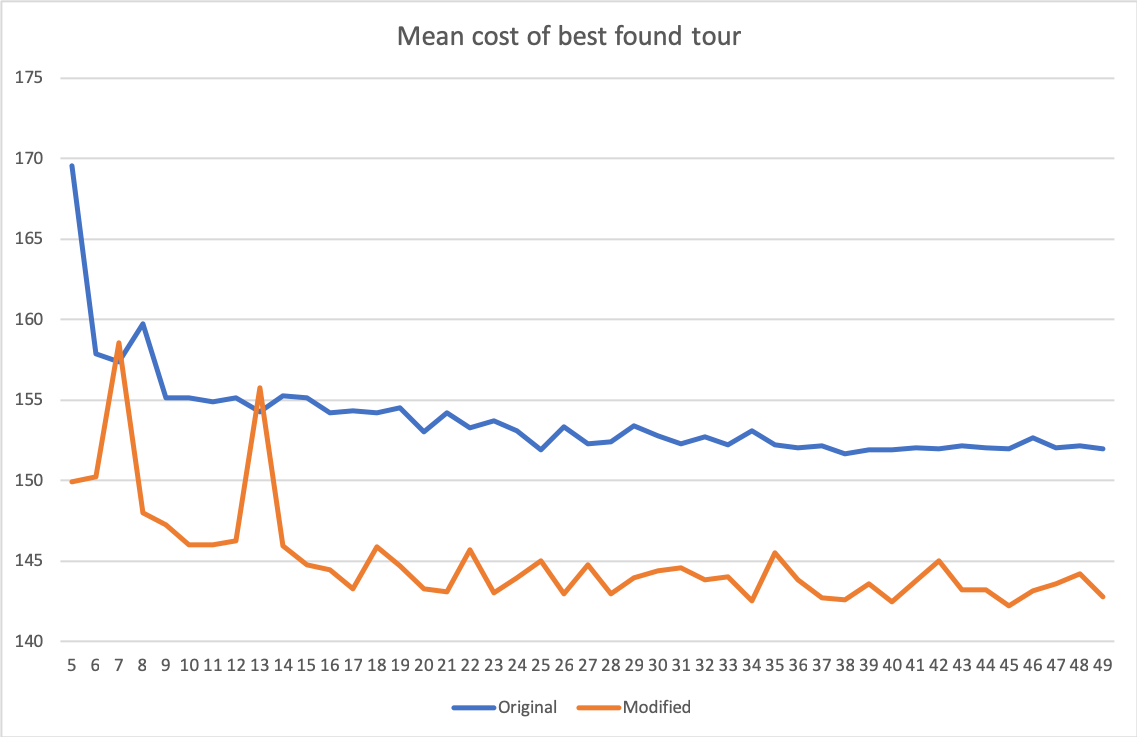
\includegraphics[width=0.9\textwidth]{candsBest.png}
	\caption{Mean costs of best found tour in relation to candidate subset size}
	\label{fig:candsBest}
\end{figure} \par

The first thing we notice in Figure \ref{fig:candsBest} is that the modified version of the algorithm outperforms the original one in this instance of the problem. That is a very positive sign for our work because it means that our assumption about the importance of rightly chosen candidates was probably right, but we will further test the quality of both methods in Section \ref{sec:length}. \par 

Another thing we can observe is that the results of the original method are a little bit more consistent than in the modified version of the algorithm. We can see this on the spikes of both methods in the graph. But this has a logical explanation, as the second method is much more dependent on the choice of the right candidate. On the contrary, when the original method chooses a candidate from some unfavorable area, there is a good chance it will more or less compensate this choice by backtracking the candidates’ optimal path and selecting a turning point which would be more prosperous for the best available path. \par For example, two major spikes in the best found tour quality found by the modified version of the algorithm when limiting the candidate set to 7 an 13 candidates are caused by this very same property of the modified algorithm. There is a tour with much better quality than others, starting at one of the origins, and the modified algorithm simply failed to find this tour at the place of these spikes, resulting in a noticeable drop in the tour quality. A similar effect can be observed on the graph of the original version of the algorithm at the mark of 8, but we see that this drop is relatively small compared to the two spikes mentioned earlier. This is the consequence of the compensation which was described above.\par The solution for the modified algorithm could be to simply select more candidates. Evidence that supports this theory could be also found in Figure \ref{fig:candsBest}. Note that the results for the modified version of the algorithm are becoming more and more consistent the more we move along the horizontal axis.\par The last conclusion we can draw from these results is the influence of the size of candidates subset to the overall performance. We see that there is a trend toward better quality with the growing size of the candidate subset. However, this trend is not by far as strong as the increase of computational resources we can see in Figure \ref{fig:candsTime}. The reason behind this is the geospatial diversity we are employing when selecting candidates into this subset. We conclude that around twenty candidates are enough to cover most of the searched area when chosen with respect to their location. This has a practical impact on the usage of the algorithm; we can define a reasonable tradeoff between the tours’ quality and the use of resources, as everything above this determined threshold would be simply ineffective with just a minor improvement of the overall tour quality.


 

\begin{figure}
	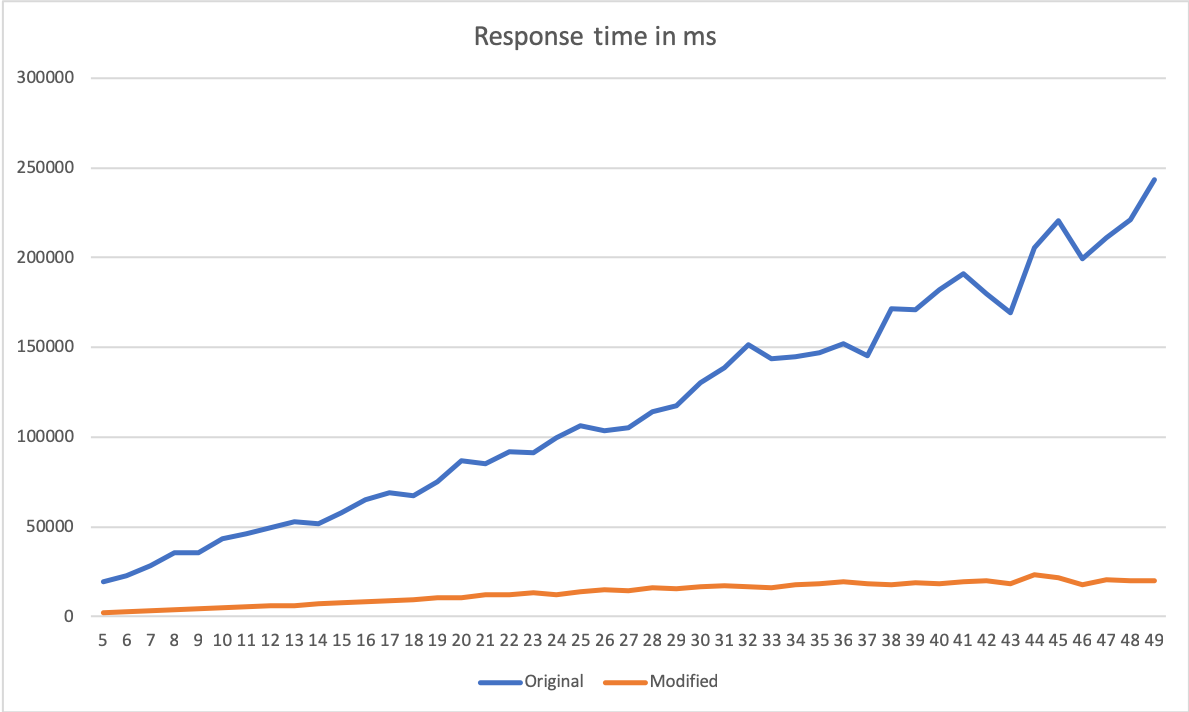
\includegraphics[width=0.9\textwidth]{candsTime.png}
	\caption{Response time of each method in relation to candidate subset size}
	\label{fig:candsTime}
\end{figure}

The last conclusion we can draw from these results is the influence of the size of candidates subset to the overall performance. We see that there is a trend toward better quality with the growing size of the candidate subset. However, this trend is not by far as strong as the increase of computational resources we can see in Figure \ref{fig:candsTime}. The reason behind this is the geospatial diversity we are employing when selecting candidates into this subset. We conclude that around twenty candidates are enough to cover most of the searched area when chosen with respect to their location. This has a practical impact on the usage of the algorithm; we can define a reasonable tradeoff between tours quality and use of resources as everything above this determined threshold would be simply ineffective with just a minor improvement of the overall tour quality.




\section{Tour Length} \label{sec:length}
The second experiment is meant to show how the algorithm and each of its versions are performing on planning shorter and longer tours.\par 
\begin{minipage}[t]{0.9\textwidth}
The setup which was used for this experiment:
\begin{itemize}
  \item Minimal length: 1000m - 22000m
  \item Maximal length: 3200m - 24200m
  \item Factor: 450
  \item Strictness: 0.9
  \item Num. of candidates: 30
\end{itemize}
\end{minipage}
\vspace{20px}


\par
Firstly, the result in the form of Figure \ref{fig:lengthBest} shows that the length of the tour specified in the input is a much more important factor influencing the tour quality then the candidate count. This is in line with our previous mentions of the influence of the road network around the origin node on the final result. \par 
Next, we can see that the results of the original and modified method are not very distinctive and that one does not prevail over another. There are lengths where the network favors the original method, and there are others favoring the modified version. This is also part of the explanation of the result in the first experiment. We see that around the length which was used in it, the modified method bears better result than the original method.
\par

\begin{figure}
	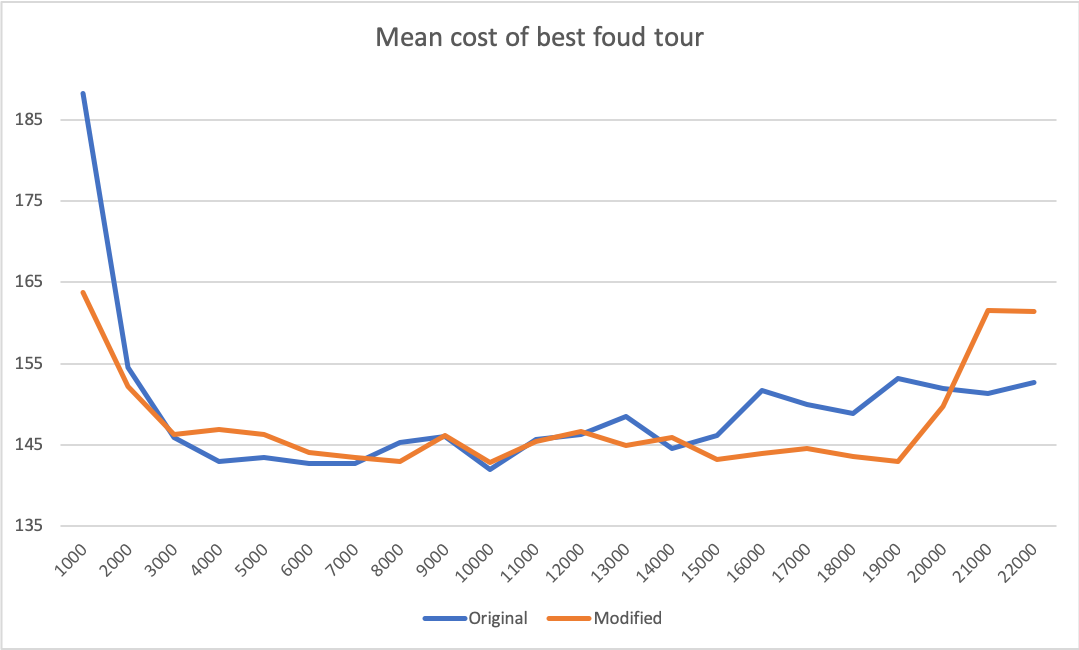
\includegraphics[width=0.9\textwidth]{lengthBest.png}
	\caption{Mean costs of best found tour in relation to lower bound of the interval}
	\label{fig:lengthBest}
\end{figure}

\begin{figure}
	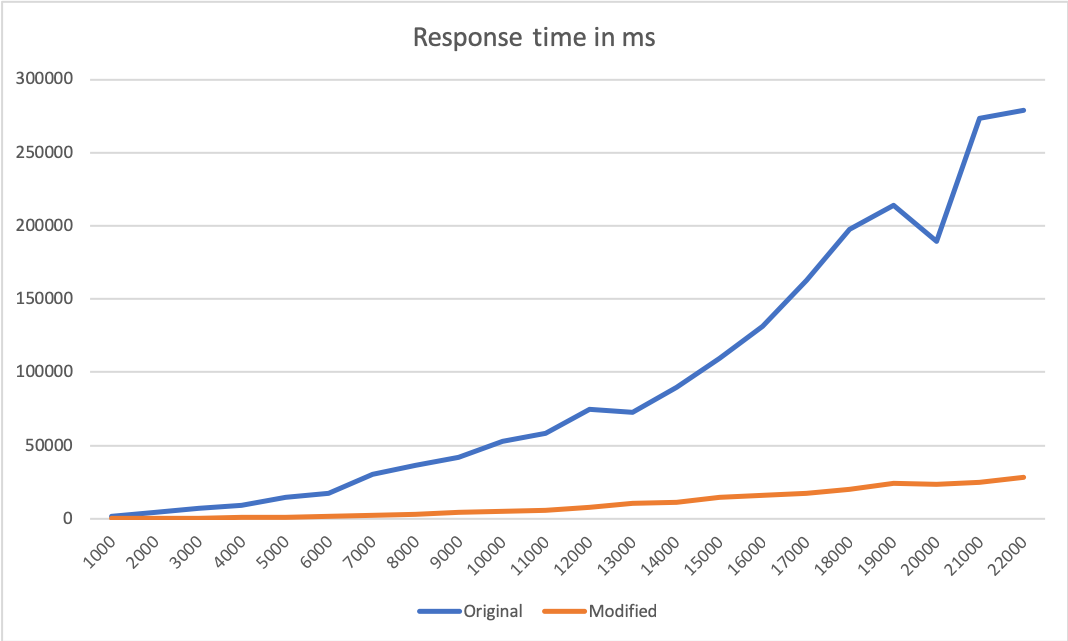
\includegraphics[width=0.9\textwidth]{lengthTime.png}
	\caption{Response time of each method in relation to lower bound of the interval}
	\label{fig:lengthTime}
\end{figure}
 \par

The average of all the best found paths in these experiment was \(149.3\) for the original method and \(147.7\) for the modified version. The lowest recorded values sit at \(142.0\) for the original and \(142.8\) for the modified version. \par
In conclusion, we see that the modifications which were done on the algorithm have their meaning. They did press down the factor with which the time of computations grows as a result of the length (as seen in Figure \ref{fig:lengthTime}). This did not affect the overall quality of its result, which are comparable and on average even slightly better than the ones from the original method.

\section{Tour Roundness} \label{sec:testRound}
The last two experiments I conducted should serve as an assurance that the input parameters which we defined as a way to control the roundness of the tour serve their purpose. Both of these experiments work with the average roundness penalty as defined in Section \ref{sec:round}. \par
Moreover, I feel like these experiments show a good example of what is the actual difference between \(\lambda\)(factor) and \(\sigma\)(strictness) as both of them are influencing the roundness, but in a different manner and reader can easily misunderstand their effects and importance. \par
As a quick sum up of relevant parts from the chapter \ref{chap:solution} where are both of these concepts described:
\begin{itemize}
\item Strictness is way to define "perfectly round tour", i.e. how far away have to two edges be to not recieve any roundness penalty
\item Factor is a way to define how great will be the recieved penalty, if the distance requirement is not satysfied 
\end{itemize}

\begin{minipage}[t]{0.9\textwidth}
The setup that both experiments share:
\begin{itemize}
  \item Minimal length: 13000m
  \item Maximal length: 16000m
  \item Num. of candidates: 20
\end{itemize}
\end{minipage}


\subsection{Factor}
This experiment, whose results are visualized in Figure \ref{fig:factorBest}, did indeed prove that the factor has an influence over the average tour roundness. \par
We can even estimate the rough interval in which this factor is an effective way to control roundness by this experiment. There is a rapid decline in the first half of the graph. This is an important finding that could be used in the later integrations of this service. To be clear, there is no way a user would know how—for him—an abstract number controls the planning and what its relation to his needs is. By estimating this interval, we can provide a more convenient control element as is, for example, a slider to let him express his wishes. In this specific case, the interval would be most convenient ranging from \(0\) to \(650\) where the average roundness penalty reaches local minima before it starts to rise again and oscillate around the mean value of \(1.77\) for the original algorithm and \(0.168\) for the modified one. \par
This result is also specific to the set of nodes used as the origin point and even more to the used graph. The planning is working with pleasantness and its values can have very distinct values in various graphs. Anyone interested in using the factor in such way should conduct a similar experiment on his own over the graph where the algorithm will be used.\par
On the other side, there is a mild spike in the average roundness penalty in the second half of the experiment. This spike can be probably explained by a smaller size of the testing sample as it contains only ten tours with the best mean cost. This makes the experiment pretty inclined to be influenced by factors such as bad choice of candidates or extremely pleasant tours with high roundness penalty. \par

\begin{figure}
	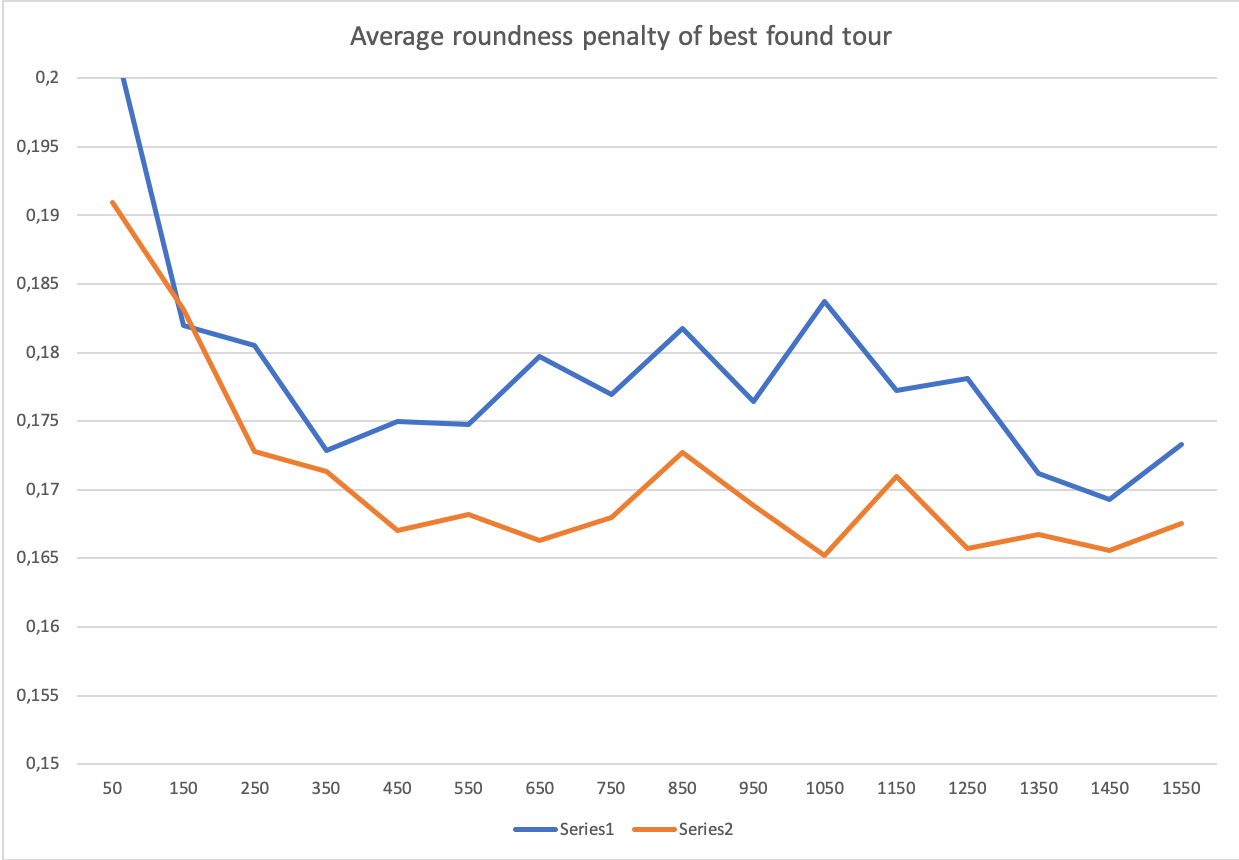
\includegraphics[width=0.9\textwidth]{factorBest.png}
	\caption{Average roundness penalty of best found tour in relation to value of \(\lambda\)}
	\label{fig:factorBest}
\end{figure}

\subsection{Strictness}
The last experiment is meant to show the influence of strictness on the tour roundness and it is successful at it. There is no continuous decline in the tour roundness, which may be confusing, but it is not an incorrect result.\par


This should give us a better insight into the results depicted in Figure \ref{fig:strictBest}. The interpretation of these results is that most of the best tours found in the first half of the experiment have such a shape that the low values of strictness have almost zero impact on them. In the first part of the experiment, the selected candidates and characteristic of the method have a far greater impact on the overall roundness than the roundness penalty and that's the reason the results are inconsistent in this part. \par
But then we observe a quick drop in the roundness penalty when the \(\sigma\) gets to \(0.7\). That's the moment when the shape of these so far planned tours does not meet this "perfectly round tour" criterion and the penalization starts to manifest itself. \par

This finding has its applications. Mainly it can be used in generic tour planning where you have no intention to let the user specify the actual strictness but merely present him with some good-looking tours. In this form of planning you are looking to fix its value to one specific number which will suit most of the users. But note that this result is specific for each graph and you should run an experiment over your graph to get this specific number.\par

\begin{figure}
	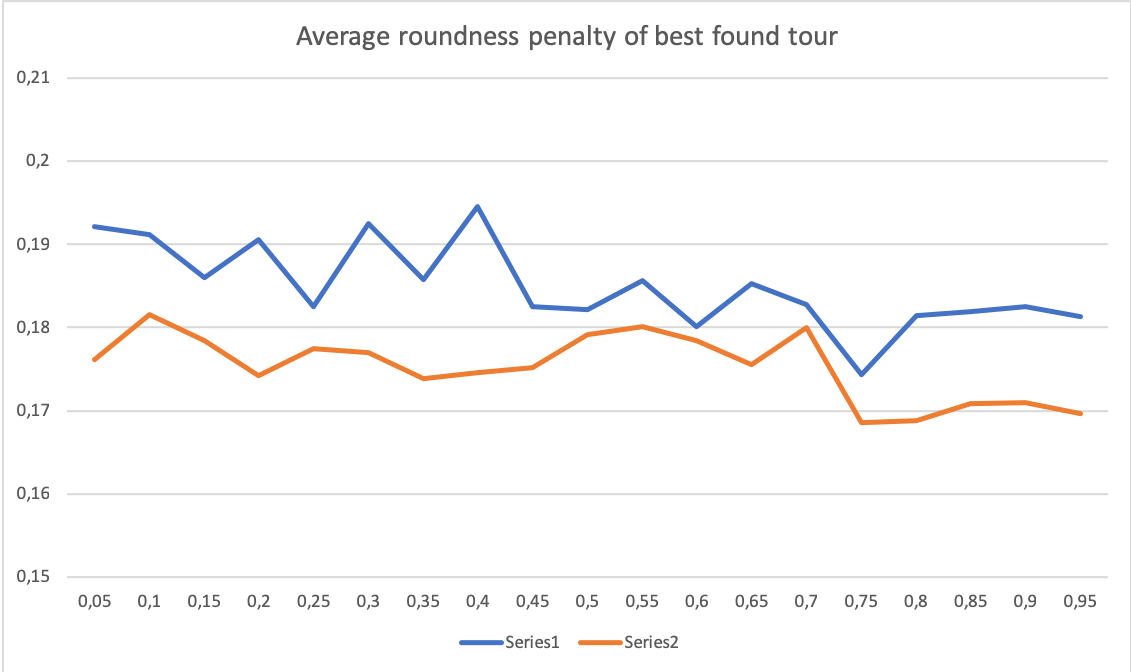
\includegraphics[width=0.9\textwidth]{strictBest.png}
	\caption{Average roundness penalty of best found tour in relation to value of \(\sigma\)}
	\label{fig:strictBest}
\end{figure}

\chapter{Conclusion}
The first and most important goal of this thesis was to find a useable solution to the problem of planning closed and point-to-point tours for recreational cycling and implement them. \par At the beginning, I defined this problem formally in a form that fit both closed as well as point-to-point recreational tours.\par After that, I researched multiple approaches to the problem and described them in detail in the opening section of this thesis. From these approaches, one particular solution called \emph{Generating Constrained Length Personalized Bicycle Tours}\cite{stroobant} was chosen as a promising base for my future work. I analyzed this solution and broke it down to the individual components as are the specification of tour roundness, forward routing, and backward routing. These components are defined in the formal way providing further insight into the problematics. \par Then I further extended the solution to solve the complete problem that I have defined at the beginning of my work by editing the roundness penalty of the tour and the forward routing stage of the original algorithm. Afterward, the second solution with the modified process of planning these tours was proposed and described in a standalone section. This modification includes multiple filters for candidate nodes found in the forward routing stage.\par Besides the theory, I also implemented both aforementioned solutions in Java. I integrated two Open Source libraries into the solution and wrote it such a way so that it be easily extendable by new search algorithms, filters, and other key parts. Moreover, the web service using REST API\cite{rest} was built on top of this implementation providing an easy way to integrate the planning of recreational tours to any application consuming this service. The last piece of software that was created for this thesis is a Javascript web client. In this client, you can customize your request for the service and consume the resulting plans. These plans are thereafter visualized over the real-world map and you can also view statistics about them in a well-arranged user interface. \par Lastly, I proposed, implemented and run multiple experiments over the utilized algorithms. These experiments were targeting various factors of the planned tours as are roundness, response time and average cost. I offer evaluation of these experiments at the end of the thesis. \par These experiments showed that there is no significant difference in the quality of tours planned by the modified version of the algorithm and the original one, but the computational time was taken down in a very significant manner.\par In the future, I plan to build on my findings and work done in this thesis and implement several more improvements into the modified version of the algorithm. The obvious choice seems to be adding the optimizations of the original solution and combining this approach with ideas from other papers mentioned above. Also, the candidate nodes filters seem to be such an effective method that it would certainly be beneficial to dive into this concept more.

\begin{thebibliography}{1}
	\bibitem{history} Cormen, T. (2009). Introduction to algorithms. Cambridge, Mass.: MIT Press.
	\bibitem{uk} GOV.UK. (2019). Government publishes £1.2 billion plan to increase cycling and walking. [online] Available at: \url{https://www.gov.uk/government/news/government-publishes-12-billion-plan-to-increase-cycling-and-walking} [Accessed 24 May 2019].
	\bibitem{eu} Mobility and Transport - European Commission. (2019). Cycling - Mobility and Transport - European Commission. [online] Available at: \url{https://ec.europa.eu/transport/themes/clean-transport-urban-transport/cycling_en} [Accessed 24 May 2019].
	\bibitem{aop} Souffriau, W., Vansteenwegen, P., Vanden Berghe, G. and Van Oudheusden, D. (2011). The planning of cycle trips in the province of East Flanders. Omega, 39(2), pp.209-213.
	\bibitem{grasp} T.A. Feo and M.G.C. Resende (1995) Greedy randomized adaptive search procedures. Journal of Global Optimization, 6:109–133, 1995.
	\bibitem{karp}Karp, R. M. (1978). \emph{A characterization of the minimum cycle mean in a digraph.} Discrete Mathematics, 23(3), 309–311. \url{https://doi.org/10.1016/0012-365x(78)90011-0} 
	\bibitem{jogging}Gemsa, A., Pajor, T., Wagner, D., \& Zündorf, T. (2013). \emph{Efficient Computation of Jogging Routes.} In Experimental Algorithms (s. 272–283). Springer Berlin Heidelberg. \url{https://doi.org/10.1007/978-3-642-38527-8_25} 
	\bibitem{bfs}Kozen, D. (2005). The design and analysis of algorithms. New York: Springer-Verlag, pp.(s. 19–20).
	\bibitem{oatsp}Maervoet, J., Brackman, P., Verbeeck, K., De Causmaecker, P., \& Vanden Berghe, G. (2013). \emph{Tour Suggestion for Outdoor Activities}. In Web and Wireless Geographical Information Systems (s. 54–63). Springer Berlin Heidelberg. \url{https://doi.org/10.1007/978-3-642-37087-8_5} 
	\bibitem{stroobant}Stroobant, P., Audenaert, P., Colle, D., \& Pickavet, M. (2018). \emph{Generating constrained length personalized bicycle tours.} 4OR, 16(4), 411–439. \url{https://doi.org/10.1007/s10288-018-0371-9} 
	\bibitem{dijkstra} E. W. Dijkstra: A note on two problems in connexion with graphs. In: Numerische Mathematik. 1 (1959), S. 269–271
	\bibitem{astar} Hart, P. E.; Nilsson, N. J.; Raphael, B. (1968). "A Formal Basis for the Heuristic Determination of Minimum Cost Paths". IEEE Transactions on Systems Science and Cybernetics SSC4. 4 (2): 100–107. \url{doi:10.1109/TSSC.1968.300136}.
	\bibitem{rest} Richardson, L. and Ruby, S. (2007). RESTful web services. Beijing: O'Reilly.
	\bibitem{git} Matocha, M., \emph{bp}, (2019), GitHub repository, \url{https://github.com/Shade254/bp}
\end{thebibliography}
\end{document}